\documentclass{article}

\usepackage[english]{babel}

% Encoding and Fonts
\usepackage[utf8]{inputenc}
\usepackage[T1]{fontenc}
\usepackage{lmodern} % Modern LaTeX font

% Page layout and typography
\usepackage[margin=0.7in]{geometry} % More balanced margin settings
\usepackage{microtype} % Subtle improvements in word spacing for aesthetics
\usepackage[parfill]{parskip}  % Space between paragraphs instead of indents

% Graphics and Colors
% \usepackage{minted}
\usepackage{graphicx}
\usepackage{subfig}
\usepackage{xcolor}
\definecolor{LightGray}{gray}{0.95}
\definecolor{colorSection}{RGB}{0, 0, 0}         
\definecolor{colorSubsection}{RGB}{0, 0, 255}     
\definecolor{colorSubsubsection}{RGB}{255, 0, 0}  
\definecolor{colorSubsubsubsection}{RGB}{0, 128, 0} 

% Hyperlinks
\usepackage[hidelinks]{hyperref} 

% Headers and Footers
\usepackage{fancyhdr}
\pagestyle{fancy}
\fancyhead{} 
\fancyfoot[C]{\thepage} 
\renewcommand{\headrulewidth}{0.5pt} 
\renewcommand{\footrulewidth}{0.5pt} 

% Math Support
\usepackage{amsmath}

% Codeblocks using listings
\usepackage{listings}
\lstdefinelanguage{Coq}{
  keywords={Definition, Inductive, Fixpoint, match, with, end, as, return, forall, exists, if, then, else, fun, Lemma, Proof, Qed, intro, intros, Theorem},
  morecomment=[s]{(*}{*)}
}
\lstdefinestyle{customc}{
  belowcaptionskip=1\baselineskip,
  breaklines=true,
  frame=L,
  xleftmargin=\parindent,
  language=Coq,
  showstringspaces=false,
  basicstyle=\footnotesize\ttfamily,
  keywordstyle=\bfseries\color{green!40!black},
  commentstyle=\itshape\color{purple!40!black},
  identifierstyle=\color{blue},
  stringstyle=\color{orange},
  backgroundcolor=\color{LightGray},
}

\definecolor{draculaBackground}{RGB}{40,42,54}
\definecolor{draculaForeground}{RGB}{248,248,242}
\definecolor{draculaComment}{RGB}{98,114,164}
\definecolor{draculaKeyword}{RGB}{139,233,253}
\definecolor{draculaFunction}{RGB}{80,250,123}
\definecolor{draculaNumber}{RGB}{189,147,249}
\definecolor{draculaString}{RGB}{241,250,140}

\lstdefinestyle{dracula}{
  belowcaptionskip=1\baselineskip,
  breaklines=true,
  frame=L,
  xleftmargin=\parindent,
  language=Coq,
  showstringspaces=false,
  basicstyle=\footnotesize\ttfamily\color{draculaForeground},
  keywordstyle=\bfseries\color{draculaKeyword},
  commentstyle=\itshape\color{draculaComment},
  identifierstyle=\color{draculaFunction},
  numberstyle=\color{draculaNumber},
  stringstyle=\color{draculaString},
  backgroundcolor=\color{draculaBackground},
}

\lstset{style=dracula}

% Lists and Enumerations
\usepackage{enumitem}
\setlist[itemize]{leftmargin=*} 

% Other utility packages
\usepackage{spverbatim}
\usepackage{cprotect}
\usepackage{lipsum}

% Title sectioning with color
\usepackage{titlesec}
\titleformat*{\section}{\large\bfseries\color{colorSection}}
\titleformat*{\subsection}{\normalsize\bfseries\color{colorSubsection}}
\titleformat*{\subsubsection}{\small\bfseries\color{colorSubsubsection}}
\titleformat{\subsubsubsection}
{\normalsize\bfseries\color{colorSubsubsubsection}}{\thesubsubsubsection}{1em}{}

\title{            
\selectfont Term Project: The Big Three in Computation - Source Interpreters, Compilers, and Virtual Machines in Arithmetic Expressions\\
\vspace{1cm}
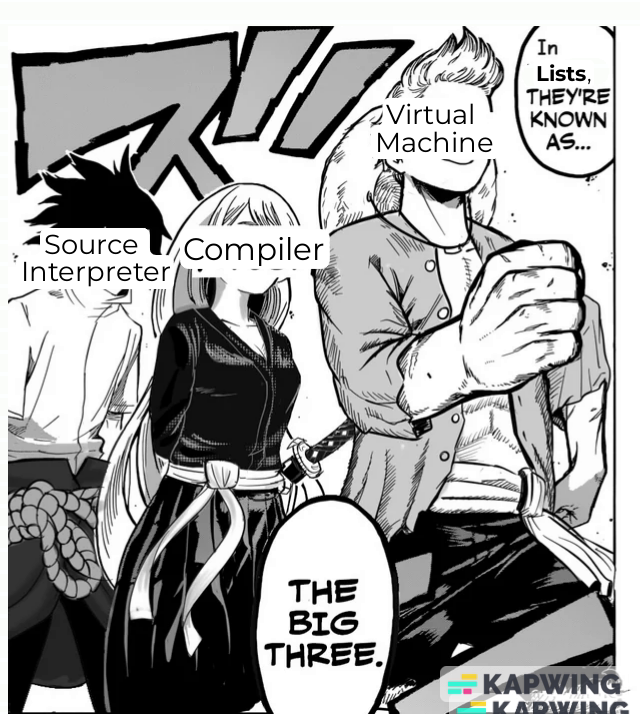
\includegraphics[width=0.8\linewidth]{Untitled_Project_V1_V2.png}
}
\author{YSC3236: Functional Programming and Proving}
\date{
  \small\emph{"The best way to understand something is to try to do it yourself."} \\
    - Olivier Danvy, during an evening walk \\
}
\begin{document}
\maketitle

\setcounter{section}{-1}

% Group member details
\newpage
\section*{Group Member Details}
\begin{itemize}
    \item Alan Matthew \\
    Email: alan.matthew@u.yale-nus.edu.sg \\
    Matriculation ID: A0224197B

    \item Jingyi Hou \\
    Email: jingyi.hou@u.yale-nus.edu.sg \\
    Matriculation ID: A0242429E

    \item Zhu Wentao \\
    Email: zhu.wentao@u.yale-nus.edu.sg \\
    Matriculation ID: A0224190N
\end{itemize}
\newpage
\tableofcontents
\newpage

\section{Introduction}
In this term project, we are asked to formalise three language processors for arithmetic expressions. Namely, we need to formalise an interpreter for arithmetic expressions, a compiler from arithmetic expressions to byte code and an interpreter for byte code (i.e., a virtual machine).

In particular, we need to prove the following theorem:

\begin{lstlisting}
Theorem the_commuting_diagram :
  forall sp : source_program,
    interpret sp = run (compile sp).
\end{lstlisting}

In other words, 

* interpreting this arithmetic expression and

* compiling this arithmetic expression and then running the resulting byte-code program

yield the same result.

While this may seem like a daunting task, we will realise through this project that we can get very far by using what we have learnt in Intro to CS and FPP. Moreover, by being relentlessly systematic in our approach, we will end up with something we can understand and explain. All these will make us more secure in our knowledge as we come to the final note of FPP.

\section{Task 1}

\subsection{Introduction}
In Task 1, we are asked to implement the two functions \texttt{evaluate} and \texttt{interpret}. Beyond that, we should prove that each of the two functions satisfies its specification. If time permitting, we are invited to prove that each specification is a unique one.  

During the live coding section of the last lecture, we have already seen the two functions implemented in continuation-passing style. As such, our implementations will be a modification of those. Apart from that, we need the property that the specification of \texttt{evaluate} is a unique one to prove that \texttt{interpret} satisfies its specification. 

The relevant specifications are as follows:

\begin{lstlisting}
(* Arithmetic expressions: *)

Inductive arithmetic_expression : Type :=
  Literal : nat -> arithmetic_expression
| Plus : arithmetic_expression -> arithmetic_expression -> arithmetic_expression
| Minus : arithmetic_expression -> arithmetic_expression -> arithmetic_expression.

(* Source programs: *)

Inductive source_program : Type :=
  Source_program : arithmetic_expression -> source_program.

(* ********** *)

(* Semantics: *)

Inductive expressible_value : Type :=
  Expressible_nat : nat -> expressible_value
| Expressible_msg : string -> expressible_value.
\end{lstlisting}

\subsection{Answer}
We first investigate the type of the \texttt{evaluate} function, which is \texttt{arithmetic\_expression -> expressible\_value}. As such, we need to first implement an equality predicate for \texttt{expressible\_value} such that we can write systematic tests for the \texttt{evaluate} function.

The equality predicate can be implemented in the following manner, making use of the equality predicates for natural numbers and strings:

\begin{lstlisting}
Definition eqb_expressible_value (ev1 ev2 : expressible_value) : bool :=
  match ev1 with
  | Expressible_nat n1 =>
      match ev2 with
      | Expressible_nat n2 =>
          eqb_nat n1 n2
      | Expressible_msg s2 =>
          false
      end
  | Expressible_msg s1 =>
      match ev2 with
      | Expressible_nat n2 =>
          false
      | Expressible_msg s2 =>
          eqb_string s1 s2
      end
  end.
\end{lstlisting}

As seen, if both \texttt{ev1} and \texttt{ev2} are of the type \texttt{Expressible\_nat}, we use the \texttt{eqb\_nat} predicate to compare the natural numbers. If both \texttt{ev1} and \texttt{ev2} are of the type \texttt{Expressible\_msg}, we use the \texttt{eqb\_string} predicate to compare the strings. Otherwise, the two are of a different type and we return false.

We can then implement tests by looking at the specification.

\begin{lstlisting}
Definition specification_of_evaluate (evaluate : arithmetic_expression -> expressible_value) :=
  (forall n : nat,
     evaluate (Literal n) = Expressible_nat n)
  /\
  ((forall (ae1 ae2 : arithmetic_expression)
           (s1 : string),
       evaluate ae1 = Expressible_msg s1 ->
       evaluate (Plus ae1 ae2) = Expressible_msg s1)
   /\
   (forall (ae1 ae2 : arithmetic_expression)
           (n1 : nat)
           (s2 : string),
       evaluate ae1 = Expressible_nat n1 ->
       evaluate ae2 = Expressible_msg s2 ->
       evaluate (Plus ae1 ae2) = Expressible_msg s2)
   /\
   (forall (ae1 ae2 : arithmetic_expression)
           (n1 n2 : nat),
       evaluate ae1 = Expressible_nat n1 ->
       evaluate ae2 = Expressible_nat n2 ->
       evaluate (Plus ae1 ae2) = Expressible_nat (n1 + n2)))
  /\
  ((forall (ae1 ae2 : arithmetic_expression)
           (s1 : string),
       evaluate ae1 = Expressible_msg s1 ->
       evaluate (Minus ae1 ae2) = Expressible_msg s1)
   /\
   (forall (ae1 ae2 : arithmetic_expression)
           (n1 : nat)
           (s2 : string),
       evaluate ae1 = Expressible_nat n1 ->
       evaluate ae2 = Expressible_msg s2 ->
       evaluate (Minus ae1 ae2) = Expressible_msg s2)
   /\
   (forall (ae1 ae2 : arithmetic_expression)
           (n1 n2 : nat),
       evaluate ae1 = Expressible_nat n1 ->
       evaluate ae2 = Expressible_nat n2 ->
       n1 <? n2 = true ->
       evaluate (Minus ae1 ae2) = Expressible_msg (String.append "numerical underflow: -" (string_of_nat (n2 - n1))))
   /\
   (forall (ae1 ae2 : arithmetic_expression)
           (n1 n2 : nat),
       evaluate ae1 = Expressible_nat n1 ->
       evaluate ae2 = Expressible_nat n2 ->
       n1 <? n2 = false ->
       evaluate (Minus ae1 ae2) = Expressible_nat (n1 - n2))).
\end{lstlisting}

In this case, we need to ensure code coverage by testing our program in an exhaustive manner. In other words, all branches within the specification should be enumerated as far as possible.

\begin{lstlisting}
Definition test_evaluate candidate :=
  (eqb_expressible_value (candidate (Literal 10)) (Expressible_nat 10))
  && (eqb_expressible_value (candidate (Plus (Literal 5) (Literal 3))) (Expressible_nat 8))
  && (eqb_expressible_value (candidate (Plus (Literal 3) (Minus (Literal 5) (Literal 8)))) (Expressible_msg "numerical underflow: -3"))
  && (eqb_expressible_value (candidate (Plus (Minus (Literal 5) (Literal 8)) (Literal 3))) (Expressible_msg "numerical underflow: -3"))
  && (eqb_expressible_value (candidate (Minus (Literal 8) (Literal 3))) (Expressible_nat 5))
  && (eqb_expressible_value (candidate (Minus (Literal 5) (Literal 8))) (Expressible_msg "numerical underflow: -3"))
  && (eqb_expressible_value (candidate (Minus (Literal 3) (Minus (Literal 5) (Literal 8)))) (Expressible_msg "numerical underflow: -3"))
  && (eqb_expressible_value (candidate (Minus (Minus (Literal 5) (Literal 8)) (Literal 3))) (Expressible_msg "numerical underflow: -3")).
\end{lstlisting}

Let us now implement the \texttt{evaluate} function proper, which is again based on its specification.

\begin{lstlisting}
Fixpoint evaluate (ae : arithmetic_expression) : expressible_value :=
  match ae with
  | Literal n =>
      Expressible_nat n
  | Plus ae1 ae2 =>
      match evaluate ae1 with
      | Expressible_nat n1 =>
          match evaluate ae2 with
          | Expressible_nat n2 =>
              Expressible_nat (n1 + n2)
          | Expressible_msg s2 =>
              Expressible_msg s2
          end
      | Expressible_msg s1 =>
          Expressible_msg s1
      end
  | Minus ae1 ae2 =>
      match evaluate ae1 with
      | Expressible_nat n1 =>
          match evaluate ae2 with
          | Expressible_nat n2 =>
              if n1 <? n2
              then Expressible_msg (String.append "numerical underflow: -" (string_of_nat (n2 - n1)))
              else Expressible_nat (n1 - n2)
          | Expressible_msg s2 =>
              Expressible_msg s2
          end
      | Expressible_msg s1 =>
          Expressible_msg s1
      end
  end.
\end{lstlisting}

The implementation is a recursive one with the \texttt{Fixpoint} notation. By aligning closely with the three cases \texttt{Literal}, \texttt{Plus} and \texttt{Minus} in the specification, we are able to complete this implementation by using match statements on the given arithmetic expressions. 

Indeed, this implementation passes the tests.

\begin{lstlisting}
Compute (test_evaluate evaluate = true).
\end{lstlisting}

However, testing only shows the presence of bugs, not their absence. We thus need to prove that the function \texttt{evaluate} satisfies its specification. 

To do that, we need to first write the fold-unfold lemmas for the \texttt{evaluate} function:

\begin{lstlisting}
Lemma fold_unfold_evaluate_Literal :
  forall (n : nat),
    evaluate (Literal n) =
      Expressible_nat n.
Proof.
  fold_unfold_tactic evaluate.
Qed.

Lemma fold_unfold_evaluate_Plus :
  forall ae1 ae2: arithmetic_expression,
    evaluate (Plus ae1 ae2) =
      match evaluate ae1 with
      | Expressible_nat n1 =>
          match evaluate ae2 with
          | Expressible_nat n2 =>
              Expressible_nat (n1 + n2)
          | Expressible_msg s =>
              Expressible_msg s
          end
      | Expressible_msg s =>
          Expressible_msg s
      end.
Proof.
  fold_unfold_tactic evaluate.
Qed.

Lemma fold_unfold_evaluate_Minus :
  forall ae1 ae2: arithmetic_expression,
    evaluate (Minus ae1 ae2) = 
      match evaluate ae1 with
      | Expressible_nat n1 =>
          match evaluate ae2 with
          | Expressible_nat n2 =>
              if n1 <? n2
              then Expressible_msg (String.append "numerical underflow: -" (string_of_nat (n2 - n1)))
              else Expressible_nat (n1 - n2)
          | Expressible_msg s =>
              Expressible_msg s
          end
      | Expressible_msg s =>
          Expressible_msg s
      end.
Proof.
   fold_unfold_tactic evaluate.
Qed.
\end{lstlisting}

As seen, there are three lemmas corresponding to the three branches of the specification.

We can then state the proposition to prove:

\begin{lstlisting}
Theorem evaluate_satisfies_the_specification_of_evaluate :
  specification_of_evaluate evaluate.
Proof.
\end{lstlisting}

The proof is routine by first unfolding \texttt{specification\_of\_evaluate} and making use of the fold-unfold lemmas specified earlier. 

\begin{lstlisting}
Theorem evaluate_satisfies_the_specification_of_evaluate :
  specification_of_evaluate evaluate.
Proof.
  unfold specification_of_evaluate.
  split.
  { intro n.
    exact (fold_unfold_evaluate_Literal n). }
  split.
  { split.
    { intros ae1 ae2 s1 S_evaluate.
      rewrite -> fold_unfold_evaluate_Plus.
      rewrite -> S_evaluate.
      reflexivity. }
    split.
    { intros ae1 ae2 n1 s2 S_evaluate SS_evaluate.
      rewrite -> fold_unfold_evaluate_Plus.
      rewrite -> S_evaluate.
      rewrite -> SS_evaluate.
      reflexivity. }
    intros ae1 ae2 n1 n2 S_evaluate SS_evaluate.
    rewrite -> fold_unfold_evaluate_Plus.
    rewrite -> S_evaluate.
    rewrite -> SS_evaluate.
    reflexivity. }
  split.
  { intros ae1 ae2 s1 S_evaluate.
    rewrite -> fold_unfold_evaluate_Minus.
    rewrite -> S_evaluate.
    reflexivity. }
  { split.
    { intros ae1 ae2 n1 s2 S_evaluate SS_evaluate.
      rewrite -> fold_unfold_evaluate_Minus.
      rewrite -> S_evaluate.
      rewrite -> SS_evaluate.
      reflexivity. }
    split.
    { intros ae1 ae2 n1 n2 S_evaluate SS_evaluate.
      rewrite -> fold_unfold_evaluate_Minus.
      rewrite -> S_evaluate.
      rewrite -> SS_evaluate.
      intro H_true.
      rewrite -> H_true.
      reflexivity. }
    intros ae1 ae2 n1 n2 S_evaluate SS_evaluate.
    rewrite -> fold_unfold_evaluate_Minus.
    rewrite -> S_evaluate.
    rewrite -> SS_evaluate.
    intro H_false.
    rewrite -> H_false.
    reflexivity. }
Qed.
\end{lstlisting}

Note here that we can use \texttt{\{\}} to ``verticalise'' our proof. This helps to keep the proof flat and ensure that it has the same structure as our program. 

Now we move on to the function \texttt{interpret}. We again begin by investigating its specification:

\begin{lstlisting}
Definition specification_of_interpret (interpret : source_program -> expressible_value) :=
  forall evaluate : arithmetic_expression -> expressible_value,
    specification_of_evaluate evaluate ->
    forall ae : arithmetic_expression,
      interpret (Source_program ae) = evaluate ae.
\end{lstlisting}

This states that for all \texttt{evaluate} functions that satisfies the specification, given any arithmetic expression, interpreting the source program of the given expression should yield the same result as evaluating the expression.

We can again begin by writing some tests for the \texttt{interpret} function:

\begin{lstlisting}
Definition test_interpret candidate :=
  (eqb_expressible_value (candidate (Source_program (Literal 10))) (Expressible_nat 10))
  && (eqb_expressible_value (candidate (Source_program (Plus (Literal 1) (Literal 10)))) (Expressible_nat 11))
  && (eqb_expressible_value (candidate (Source_program (Plus (Literal 1) (Minus (Literal 9) (Literal 10))))) (Expressible_msg "numerical underflow: -1"))
  && (eqb_expressible_value (candidate (Source_program (Plus (Minus (Literal 9) (Literal 10)) (Literal 1)))) (Expressible_msg "numerical underflow: -1"))
  && (eqb_expressible_value (candidate (Source_program (Minus (Literal 10) (Literal 1)))) (Expressible_nat 9))
  && (eqb_expressible_value (candidate (Source_program (Minus (Literal 1) (Literal 10)))) (Expressible_msg "numerical underflow: -9"))
  && (eqb_expressible_value (candidate (Source_program (Minus (Literal 1) (Minus (Literal 9) (Literal 10))))) (Expressible_msg "numerical underflow: -1"))
  && (eqb_expressible_value (candidate (Source_program (Minus (Minus (Literal 9) (Literal 10)) (Literal 1)))) (Expressible_msg "numerical underflow: -1")).
\end{lstlisting}

Note that the tests are very similar to those written for the \texttt{evaluate} function. 

The implementation of \texttt{interpret} is straightforward by making use of the \texttt{evaluate} function:

\begin{lstlisting}
Definition interpret (sp : source_program) : expressible_value :=
  match sp with
    Source_program ae =>
      evaluate ae
  end.
\end{lstlisting}

Indeed, this implementation passes the tests.

\begin{lstlisting}
Compute (test_interpret interpret = true).
\end{lstlisting}

Similar to before, we need to prove that our implementation satisfies the specification of \texttt{interpret}.

To do that, we need an Eureka lemma which states that there is at most one \texttt{interpret} function. 

\begin{lstlisting}
Theorem there_is_at_most_one_evaluate_function :
  forall (evaluate0 evaluate1 : arithmetic_expression -> expressible_value),
    specification_of_evaluate evaluate0 ->
    specification_of_evaluate evaluate1 ->
    forall ae : arithmetic_expression,
      evaluate0 ae = evaluate1 ae.
Proof.
\end{lstlisting}

The proof is by induction, making use of the fold-unfold lemmas for \texttt{evaluate}. One also need to take great care when using the \texttt{destruct} tactic by naming all relevant terms. Tactics such as \texttt{injection} and \texttt{f\_equal} also come handy in this proof. The entire proof is as follows:

\begin{lstlisting}
Theorem there_is_at_most_one_evaluate_function :
  forall (evaluate0 evaluate1 : arithmetic_expression -> expressible_value),
    specification_of_evaluate evaluate0 ->
    specification_of_evaluate evaluate1 ->
    forall ae : arithmetic_expression,
      evaluate0 ae = evaluate1 ae.
Proof.
  intros evaluate1 evaluate2.
  intros S_evaluate1 S_evaluate2.
  intro ae.
  induction ae as [n | ae1 IHae1 ae2 IHae2 | ae1 IHae1 ae2 IHae2].
  + unfold specification_of_evaluate in S_evaluate1.
    destruct S_evaluate1 as [fold_unfold_evaluate1_Literal _].
    unfold specification_of_evaluate in S_evaluate2.
    destruct S_evaluate2 as [fold_unfold_evaluate2_Literal _].
    rewrite -> (fold_unfold_evaluate1_Literal n).
    rewrite -> (fold_unfold_evaluate2_Literal n).
    reflexivity.
  + case (evaluate1 ae1) as [n11 | s11] eqn:E1_ae1;
      case (evaluate2 ae1) as [n21 | s21] eqn:E2_ae1;
      case (evaluate1 ae2) as [n12 | s12] eqn:E1_ae2;
      case (evaluate2 ae2) as [n22 | s22] eqn:E2_ae2.
    ++ destruct S_evaluate1 as [_ [[_ [_ fold_unfold_evaluate1_Plus]] _]].
       destruct S_evaluate2 as [_ [[_ [_ fold_unfold_evaluate2_Plus]] _]].
       Check (fold_unfold_evaluate1_Plus ae1 ae2 n11 n12).
       Check (fold_unfold_evaluate1_Plus ae1 ae2 n11 n12 E1_ae1 E1_ae2).
       rewrite -> (fold_unfold_evaluate1_Plus ae1 ae2 n11 n12 E1_ae1 E1_ae2).
       Check (fold_unfold_evaluate2_Plus ae1 ae2).
       Check (fold_unfold_evaluate2_Plus ae1 ae2 n21 n22).
       Check (fold_unfold_evaluate2_Plus ae1 ae2 n21 n22 E2_ae1 E2_ae2).
       rewrite -> (fold_unfold_evaluate2_Plus ae1 ae2 n21 n22 E2_ae1 E2_ae2).
       injection IHae1 as H_eq_n11_n21.
       rewrite -> H_eq_n11_n21.
       injection IHae2 as H_eq_n12_n22.
       rewrite -> H_eq_n12_n22.
       reflexivity.
    ++ discriminate IHae2.
    ++ discriminate IHae2.
    ++ unfold specification_of_evaluate in S_evaluate1.
       destruct S_evaluate1 as [_ [[_ [fold_unfold_evaluate1_Plus _]] _]].
       destruct S_evaluate2 as [_ [[_ [fold_unfold_evaluate2_Plus _]] _]].
       Check (fold_unfold_evaluate1_Plus ae1 ae2 n11 s12 E1_ae1 E1_ae2).
       rewrite -> (fold_unfold_evaluate1_Plus ae1 ae2 n11 s12 E1_ae1 E1_ae2).
       Check (fold_unfold_evaluate2_Plus ae1 ae2 n21 s22 E2_ae1 E2_ae2).
       rewrite -> (fold_unfold_evaluate2_Plus ae1 ae2 n21 s22 E2_ae1 E2_ae2).
       injection IHae2 as H_eq_s12_s22.
       Check (f_equal Expressible_msg H_eq_s12_s22).
       exact (f_equal Expressible_msg H_eq_s12_s22).
    ++ discriminate IHae1.
    ++ discriminate IHae1.
    ++ discriminate IHae1.
    ++ discriminate IHae1.
    ++ discriminate IHae1.
    ++ discriminate IHae1.
    ++ discriminate IHae1.
    ++ discriminate IHae1.
    ++ unfold specification_of_evaluate in S_evaluate1.
       destruct S_evaluate1 as [_ [[fold_unfold_evaluate1_Plus _] _]].
       destruct S_evaluate2 as [_ [[fold_unfold_evaluate2_Plus _] _]].
       Check (fold_unfold_evaluate1_Plus ae1 ae2 s11 E1_ae1).
       rewrite -> (fold_unfold_evaluate1_Plus ae1 ae2 s11 E1_ae1).
       Check (fold_unfold_evaluate2_Plus ae1 ae2 s21 E2_ae1).
       rewrite -> (fold_unfold_evaluate2_Plus ae1 ae2 s21 E2_ae1).
       injection IHae1 as H_eq_s11_s21.
       rewrite -> H_eq_s11_s21.
       reflexivity.
    ++ discriminate IHae2.
    ++ discriminate IHae2.
    ++ unfold specification_of_evaluate in S_evaluate1.
       destruct S_evaluate1 as [_ [[fold_unfold_evaluate1_Plus _] _]].
       destruct S_evaluate2 as [_ [[fold_unfold_evaluate2_Plus _] _]].
       rewrite -> (fold_unfold_evaluate1_Plus ae1 ae2 s11 E1_ae1).
       rewrite -> (fold_unfold_evaluate2_Plus ae1 ae2 s21 E2_ae1).
       injection IHae1 as H_eq_s11_s21.
       rewrite -> H_eq_s11_s21.
       reflexivity.
  + case (evaluate1 ae1) as [n11 | s11] eqn:E1_ae1;
      case (evaluate2 ae1) as [n21 | s21] eqn:E2_ae1;
      case (evaluate1 ae2) as [n12 | s12] eqn:E1_ae2;
      case (evaluate2 ae2) as [n22 | s22] eqn:E2_ae2.
    ++ case (n11 <? n12) eqn: H_n11_lt_n12;
         case (n21 <? n22) eqn: H_n21_lt_n22.
       +++ destruct S_evaluate1 as [_ [_ [_ [_ [fold_unfold_evaluate1_Minus_lt _]]]]].
           destruct S_evaluate2 as [_ [_ [_ [_ [fold_unfold_evaluate2_Minus_lt _]]]]].
           Check (fold_unfold_evaluate1_Minus_lt ae1 ae2 n11 n12 E1_ae1 E1_ae2).
           Check (fold_unfold_evaluate1_Minus_lt ae1 ae2 n11 n12 E1_ae1 E1_ae2 H_n11_lt_n12).
           rewrite -> (fold_unfold_evaluate1_Minus_lt ae1 ae2 n11 n12 E1_ae1 E1_ae2 H_n11_lt_n12).
           rewrite -> (fold_unfold_evaluate2_Minus_lt ae1 ae2 n21 n22 E2_ae1 E2_ae2 H_n21_lt_n22).
           injection IHae1 as H_eq_n11_n21.
           rewrite -> H_eq_n11_n21.
           injection IHae2 as H_eq_n21_n22.
           rewrite -> H_eq_n21_n22.
           reflexivity.
       +++ injection IHae1 as H_eq_n11_n21.
           injection IHae2 as H_eq_n12_n22.
           rewrite -> H_eq_n11_n21 in H_n11_lt_n12.
           rewrite <- H_eq_n12_n22 in H_n21_lt_n22.
           rewrite -> H_n11_lt_n12 in H_n21_lt_n22.
           discriminate H_n21_lt_n22.
       +++ injection IHae1 as H_eq_n11_n21.
           injection IHae2 as H_eq_n12_n22.
           rewrite -> H_eq_n11_n21 in H_n11_lt_n12.
           rewrite <- H_eq_n12_n22 in H_n21_lt_n22.
           rewrite -> H_n11_lt_n12 in H_n21_lt_n22.
           discriminate H_n21_lt_n22.
       +++ destruct S_evaluate1 as [_ [_ [_ [_ [_ fold_unfold_evaluate1_Minus_gt]]]]].
           destruct S_evaluate2 as [_ [_ [_ [_ [_ fold_unfold_evaluate2_Minus_gt]]]]].
           Check (fold_unfold_evaluate1_Minus_gt ae1 ae2 n11 n12 E1_ae1 E1_ae2 H_n11_lt_n12).
           rewrite -> (fold_unfold_evaluate1_Minus_gt ae1 ae2 n11 n12 E1_ae1 E1_ae2 H_n11_lt_n12).
           rewrite -> (fold_unfold_evaluate2_Minus_gt ae1 ae2 n21 n22 E2_ae1 E2_ae2 H_n21_lt_n22).
           injection IHae1 as H_eq_n11_n21.
           injection IHae2 as H_eq_n12_n22.
           rewrite -> H_eq_n11_n21.
           rewrite -> H_eq_n12_n22.
           reflexivity.
    ++ discriminate IHae2.
    ++ discriminate IHae2.
    ++ destruct S_evaluate1 as [_ [_ [_ [fold_unfold_evaluate1_Minus _]]]].
       destruct S_evaluate2 as [_ [_ [_ [fold_unfold_evaluate2_Minus _]]]].
       Check (fold_unfold_evaluate1_Minus ae1 ae2 n11 s12 E1_ae1 E1_ae2).
       rewrite -> (fold_unfold_evaluate1_Minus ae1 ae2 n11 s12 E1_ae1 E1_ae2).
       rewrite -> (fold_unfold_evaluate2_Minus ae1 ae2 n21 s22 E2_ae1 E2_ae2).
       injection IHae2 as H_eq_s12_s22.
       rewrite -> H_eq_s12_s22.
       reflexivity.
    ++ discriminate IHae1.
    ++ discriminate IHae1.
    ++ discriminate IHae1.
    ++ discriminate IHae1.
    ++ discriminate IHae1.
    ++ discriminate IHae1.
    ++ discriminate IHae1.
    ++ discriminate IHae1.
    ++ destruct S_evaluate1 as [_ [_ [fold_unfold_evaluate1_Minus _]]].
       destruct S_evaluate2 as [_ [_ [fold_unfold_evaluate2_Minus _]]].
       Check (fold_unfold_evaluate1_Minus ae1 ae2 s11 E1_ae1).
       rewrite -> (fold_unfold_evaluate1_Minus ae1 ae2 s11 E1_ae1).
       rewrite -> (fold_unfold_evaluate2_Minus ae1 ae2 s21 E2_ae1).
       injection IHae1 as H_eq_s11_s21.
       rewrite -> H_eq_s11_s21.
       reflexivity.
    ++ discriminate IHae2.
    ++ discriminate IHae2.
    ++ destruct S_evaluate1 as [_ [_ [fold_unfold_evaluate1_Minus _]]].
       destruct S_evaluate2 as [_ [_ [fold_unfold_evaluate2_Minus _]]].
       Check (fold_unfold_evaluate1_Minus ae1 ae2 s11 E1_ae1).
       rewrite -> (fold_unfold_evaluate1_Minus ae1 ae2 s11 E1_ae1).
       rewrite -> (fold_unfold_evaluate2_Minus ae1 ae2 s21 E2_ae1).
       injection IHae1 as H_eq_s11_s21.
       rewrite -> H_eq_s11_s21.
       reflexivity.
Qed.
\end{lstlisting}

With this, the proof that our implementation satisfies the specification of \texttt{interpret} can be done in an elegant manner using the \texttt{exact} tactic:

\begin{lstlisting}
Theorem interpret_satisfies_the_specification_of_interpret :
  specification_of_interpret interpret.
Proof.
  unfold specification_of_interpret, interpret.
  intros evaluate0 S_evaluate0 ae.
  Check (there_is_at_most_one_evaluate_function evaluate evaluate0 evaluate_satisfies_the_specification_of_evaluate S_evaluate0 ae).
  exact (there_is_at_most_one_evaluate_function evaluate evaluate0 evaluate_satisfies_the_specification_of_evaluate S_evaluate0 ae).
Qed.
\end{lstlisting}

Furthermore, as an extra, we can also prove that there is also at most one interpret function:

Here, we must take care to handle \texttt{sp} of type \texttt{source\_program} appropriately. Since the type \texttt{source\_program} is an inductive type with only one constructor, we can use the \texttt{case} tactic to destruct \texttt{sp} into its constituent parts, namely an arithmetic expression \texttt{ae}.

\begin{lstlisting}
Theorem there_is_at_most_one_interpret_function :
  forall interpret1 interpret2 : source_program -> expressible_value,
    specification_of_interpret interpret1 ->
    specification_of_interpret interpret2 ->
    forall sp : source_program,
      interpret1 sp = interpret2 sp.
Proof.
  intros interpret1 interpret2 S_interpret1 S_interpret2.
  unfold specification_of_interpret in S_interpret1.
  unfold specification_of_interpret in S_interpret2.
  case sp as [ae].
  Check (S_interpret1 evaluate evaluate_satisfies_the_specification_of_evaluate ae).
  rewrite -> (S_interpret1 evaluate evaluate_satisfies_the_specification_of_evaluate ae).
  rewrite -> (S_interpret2 evaluate evaluate_satisfies_the_specification_of_evaluate ae).
  reflexivity.
Qed.
\end{lstlisting}

The remainder of the proof is routine as long as we remain constantly vigilant in applying our assumptions and lemmas appropriately.
    
\subsection{Conclusion}
To conclude this task, we have implemented the \texttt{evaluate} and \texttt{interpret} functions based on their respective specifications. To test our implementation, we have also implemented the equality predicate for \texttt{expressible\_value}. Last but not least, we prove that our implementations satisfy their respective specifications.

Doing this is a reminder that to make use of what we know and realise how much it scales. Indeed, much of what we have learnt in Intro to CS and FPP comes in handy in solving this task alone. 

\section{Task 2}

\subsection{Introduction}
In Task 2, we are asked to implement \texttt{decode\_execute} given its informal specification. In particular, the specification has three cases to consider: PUSH, ADD and SUB. For PUSH, any natural number \texttt{n} can be pushed to the stack \texttt{ds}. For ADD, there are two scenarios depending on whether the stack contains at least two natural numbers. For SUB, there is an additional case if subtracting one natural number from the other gives a negative result.  

The relevant specifications are as follows:

\begin{lstlisting}

(* Byte-code instructions: *)

Inductive byte_code_instruction : Type :=
  PUSH : nat -> byte_code_instruction
| ADD : byte_code_instruction
| SUB : byte_code_instruction.

(* Target programs: *)

Inductive target_program : Type :=
  Target_program : list byte_code_instruction -> target_program.

(* Data stack: *)

Definition data_stack := list nat.

(* ********** *)

Inductive result_of_decoding_and_execution : Type :=
  OK : data_stack -> result_of_decoding_and_execution
| KO : string -> result_of_decoding_and_execution.

\end{lstlisting}
    
\subsection{Answer}
We first investigate the type of the \texttt{decode\_execute} function.

Observing our function, it gives a result of the type \texttt{result\_of\_decoding\_and\_execution}. As such, we need to first implement an equality predicate for \texttt{result\_of\_decoding\_and\_execution} such that we can write systematic tests for the \texttt{decode\_execute} function.

To do that, we first need to implement an equality predicate for \texttt{data\_stack}.

\begin{lstlisting}
Definition eqb_data_stack (ds1 ds2 : list nat) : bool :=
  eqb_list nat eqb_nat ds1 ds2.
\end{lstlisting}

The equality predicate for \texttt{result\_of\_decoding\_and\_execution} can then be implemented in the following manner:

\begin{lstlisting}
Definition eqb_result_of_decoding_and_execution (res1 res2 : result_of_decoding_and_execution) : bool :=
  match res1 with
  | OK ds1 =>
      match res2 with
      | OK ds2 =>
          eqb_data_stack ds1 ds2
      | KO msg2 =>
          false
      end
  | KO msg1 =>
      match res2 with
      | OK ds2 =>
          false
      | KO msg2 =>
          eqb_string msg1 msg2
      end
  end.
\end{lstlisting}

As seen, if both \texttt{res1} and \texttt{res2} are of the type \texttt{OK}, we use the \texttt{eqb\_data\_stack} predicate to compare the data stacks. If both \texttt{res1} and \texttt{res2} are of the type \texttt{KO}, we use the \texttt{eqb\_string} predicate to compare the strings. Otherwise, the two are of a different type and we return false.

We can then implement tests by looking at the specification. In this case, we are not given a formal specification. Rather, the informal specification is written in prose. 

\begin{lstlisting}
Definition test_decode_execute candidate :=
  (eqb_result_of_decoding_and_execution (candidate (PUSH 4) (3 :: 2 :: 1 :: nil)) (OK (4 :: 3 :: 2 :: 1 :: nil)))
  && (eqb_result_of_decoding_and_execution (candidate ADD nil) (KO "ADD: stack underflow"))
  && (eqb_result_of_decoding_and_execution (candidate ADD (1 :: nil)) (KO "ADD: stack underflow"))
  && (eqb_result_of_decoding_and_execution (candidate ADD (2 :: 1 :: nil)) (OK (3 :: nil)))
  && (eqb_result_of_decoding_and_execution (candidate ADD (3 :: 2 :: 1 :: nil)) (OK (5 :: 1 :: nil)))
  && (eqb_result_of_decoding_and_execution (candidate SUB nil) (KO "SUB: stack underflow"))
  && (eqb_result_of_decoding_and_execution (candidate SUB (1 :: nil)) (KO "SUB: stack underflow"))
  && (eqb_result_of_decoding_and_execution (candidate SUB (2 :: 1 :: nil)) (KO "numerical underflow: -1"))
  && (eqb_result_of_decoding_and_execution (candidate SUB (1 :: 2 :: nil)) (OK (1 :: nil)))
  && (eqb_result_of_decoding_and_execution (candidate SUB (1 :: 2 :: 3 :: 4 :: nil)) (OK (1 :: 3 :: 4 :: nil))).
\end{lstlisting}

Similarly, we need to ensure code coverage by testing our program in an exhaustive manner. In other words, all branches within the specification should be enumerated as far as possible.

There are three cases to consider as laid out in the introduction. The function can thus be implemented in the following way:

\begin{lstlisting}
Definition decode_execute (bci : byte_code_instruction) (ds : data_stack) : result_of_decoding_and_execution :=
  match bci with
  | PUSH n =>
      OK (n :: ds)
  | ADD =>
      match ds with
      | nil =>
          KO "ADD: stack underflow"
      | n2 :: ds' =>
          match ds' with
          | nil =>
              KO "ADD: stack underflow"
          | n1 :: ds'' =>
              OK ((n1 + n2) :: ds'')
          end
      end
  | SUB =>
      match ds with
      | nil =>
          KO "SUB: stack underflow"
      | n2 :: ds' =>
          match ds' with
          | nil =>
              KO "SUB: stack underflow"
          | n1 :: ds'' =>
              if n1 <? n2 
              then KO (String.append "numerical underflow: -" (string_of_nat (n2 - n1)))
              else OK ((n1 - n2) :: ds'')
          end
      end
  end.
\end{lstlisting}

Note that we need to take care of the ordering in which the elements are being processed. In particular, the second element \texttt{n2} is processed first in both the \texttt{ADD} and \texttt{SUB} cases.

Indeed, this implementation passes the tests.

\begin{lstlisting}
Compute (test_decode_execute decode_execute = true).
\end{lstlisting}

\subsection{Conclusion}
In this task, a key takeaway is to understand what the program does before writing down an implementation. In particular, we need to understand how elements are processed during decoding and execution to come up with a sensible naming convention. 

\section{Task 3}

\subsection{Introduction}
In Task 3, we are asked to implement the recursive function \texttt{fetch\_decode\_execute\_loop}. In this case, we are given its formal specification as follows:

\begin{lstlisting}
Definition specification_of_fetch_decode_execute_loop (fetch_decode_execute_loop : list byte_code_instruction -> data_stack -> result_of_decoding_and_execution) :=
  (forall ds : data_stack,
      fetch_decode_execute_loop nil ds = OK ds)
  /\
  (forall (bci : byte_code_instruction)
          (bcis' : list byte_code_instruction)
          (ds ds' : data_stack),
      decode_execute bci ds = OK ds' ->
      fetch_decode_execute_loop (bci :: bcis') ds =
      fetch_decode_execute_loop bcis' ds')
  /\
  (forall (bci : byte_code_instruction)
          (bcis' : list byte_code_instruction)
          (ds : data_stack)
          (s : string),
      decode_execute bci ds = KO s ->
      fetch_decode_execute_loop (bci :: bcis') ds =
      KO s).
\end{lstlisting}

We are then asked that our implementation satisfies the specification of \texttt{fetch\_decode\_execute\_loop}. If time permitting, we are invited to prove that the specification is a unique one.  

\subsection{Answer}
Similar to Task 1, we can prove that there is at most one \texttt{fetch\_decode\_execute\_loop} by induction: 

\begin{lstlisting}
Theorem there_is_at_most_one_fetch_decode_execute_loop :
  forall
    (fdel1 fdel2 : list byte_code_instruction -> data_stack -> result_of_decoding_and_execution)
    (bcis : list byte_code_instruction)
    (ds : data_stack),
    specification_of_fetch_decode_execute_loop fdel1 ->
    specification_of_fetch_decode_execute_loop fdel2 ->
    fdel1 bcis ds = fdel2 bcis ds.
Proof.
  intros fdel1 fdel2 bcis.
  induction bcis as [ | bci bcis' IHbcis' ]; intro ds.
  + unfold specification_of_fetch_decode_execute_loop.
    intros S_fdel1 S_fdel2.
    destruct S_fdel1 as [H_fdel1_nil_OK _].
    destruct S_fdel2 as [H_fdel2_nil_OK _].
    rewrite -> H_fdel1_nil_OK.
    rewrite -> H_fdel2_nil_OK.
    reflexivity.
  + intros S_fdel1 S_fdel2.
    assert (H_fdel1 := S_fdel1).
    assert (H_fdel2 := S_fdel2).
    unfold specification_of_fetch_decode_execute_loop in H_fdel1.
    unfold specification_of_fetch_decode_execute_loop in H_fdel2.
    destruct H_fdel1 as [_ [H_fdel1_OK H_fdel1_KO]].
    destruct H_fdel2 as [_ [H_fdel2_OK H_fdel2_KO]].
    Check (decode_execute bci ds).
    case (decode_execute bci ds) as [OK_ds | KO_s] eqn: H_de_OK_ds.
   { Check (H_fdel1_OK bci bcis' ds).
       Check (H_fdel1_OK bci bcis' ds OK_ds H_de_OK_ds).
       rewrite -> (H_fdel1_OK bci bcis' ds OK_ds H_de_OK_ds).
       rewrite -> (H_fdel2_OK bci bcis' ds OK_ds H_de_OK_ds).
       Check (IHbcis' OK_ds S_fdel1 S_fdel2).
       exact (IHbcis' OK_ds S_fdel1 S_fdel2). }
   { Check (H_fdel1_KO bci bcis' ds).
       Check (H_fdel1_KO bci bcis' ds KO_s H_de_OK_ds).
       rewrite -> (H_fdel1_KO bci bcis' ds KO_s H_de_OK_ds).
       rewrite -> (H_fdel2_KO bci bcis' ds KO_s H_de_OK_ds).
       reflexivity. }
Qed.
\end{lstlisting}

We can then implement tests by looking at the specification of \texttt{fetch\_decode\_execute\_loop}. As usual, code coverage is important here. 

\begin{lstlisting}
Definition test_fetch_decode_execute_loop candidate :=
  (eqb_result_of_decoding_and_execution (candidate nil (3 :: 2 :: 1 :: nil)) (OK (3 :: 2 :: 1 :: nil)))
  && (eqb_result_of_decoding_and_execution (candidate ((PUSH 3) :: (PUSH 4) :: nil) (2 :: 1 :: nil)) (OK (4 :: 3 :: 2 :: 1 :: nil)))
  && (eqb_result_of_decoding_and_execution (candidate (ADD :: (PUSH 2) :: nil) nil) (KO "ADD: stack underflow"))
  && (eqb_result_of_decoding_and_execution (candidate (ADD :: (PUSH 2) :: nil) (1 :: nil)) (KO "ADD: stack underflow"))
  && (eqb_result_of_decoding_and_execution (candidate (SUB :: (PUSH 2) :: nil) (1 :: nil)) (KO "SUB: stack underflow"))
  && (eqb_result_of_decoding_and_execution (candidate (SUB :: (PUSH 3) :: nil) (2 :: 1 :: nil)) (KO "numerical underflow: -1"))
  && (eqb_result_of_decoding_and_execution (candidate (SUB :: (PUSH 10) :: nil) (1 :: 2 :: nil)) (OK (10 :: 1 :: nil)))
  && (eqb_result_of_decoding_and_execution (candidate (SUB :: (PUSH 10) :: nil) (1 :: 2 :: 100 :: nil)) (OK (10 :: 1 :: 100 :: nil))).
\end{lstlisting}

Based on the specification, we can implement the function in the following manner:

\begin{lstlisting}
Fixpoint fetch_decode_execute_loop (bcis : list byte_code_instruction) (ds : data_stack) : result_of_decoding_and_execution :=
  match bcis with
  | nil =>
      OK ds
  | bci :: bcis' =>
      match decode_execute bci ds with
      | OK ds' =>
          fetch_decode_execute_loop bcis' ds'
      | KO s =>
          KO s
      end
  end.
\end{lstlisting}

As seen, the function is recursive with the \texttt{Fixpoint} notation. Depending on whether the list of byte code instruction is empty, we have two branches. In the second branch, we again separate into two branches depending on whether decoding and executing the first instruction on the data stack yields a result of type \texttt{OK} or \texttt{KO}.

Indeed, this implementation passes the tests.

\begin{lstlisting}
Compute (test_fetch_decode_execute_loop fetch_decode_execute_loop = true).
\end{lstlisting}

However, testing only shows the presence of bugs, not their absence. We thus need to prove that the function \texttt{fetch\_decode\_execute\_loop} satisfies its specification. 

To do that, we need to first write the fold-unfold lemmas for the \texttt{fetch\_decode\_execute\_loop} function:

\begin{lstlisting}
Lemma fold_unfold_fetch_decode_execute_nil:
  forall (ds : data_stack),
    fetch_decode_execute_loop nil ds =
      OK ds.
Proof.
  fold_unfold_tactic fetch_decode_execute_loop.
Qed.

Lemma fold_unfold_fetch_decode_execute_cons:
  forall (ds : data_stack)
         (bci : byte_code_instruction)
         (bcis' : list byte_code_instruction),
    fetch_decode_execute_loop (bci :: bcis') ds =
      match decode_execute bci ds with
      | OK ds' =>
          fetch_decode_execute_loop bcis' ds'
      | KO s =>
          KO s
      end.
Proof.
  fold_unfold_tactic fetch_decode_execute_loop.
Qed.
\end{lstlisting}

We can then state the proposition to prove:

\begin{lstlisting}
Theorem fetch_decode_execute_loop_satisfies_the_specification_of_fetch_decode_execute_loop :
  specification_of_fetch_decode_execute_loop fetch_decode_execute_loop.
Proof.
\end{lstlisting}

The proof is routine by first unfolding \texttt{specification\_of\_fetch\_decode\_execute\_loop} and making use of the fold-unfold lemmas specified earlier. 

\begin{lstlisting}
Theorem fetch_decode_execute_loop_satisfies_the_specification_of_fetch_decode_execute_loop :
  specification_of_fetch_decode_execute_loop fetch_decode_execute_loop.
Proof.
  unfold specification_of_fetch_decode_execute_loop.
  split.
  { exact fold_unfold_fetch_decode_execute_nil. }
  split.
    { intros bci bcis' ds ds' S_decode_execute_loop.
      rewrite -> fold_unfold_fetch_decode_execute_cons.
      rewrite -> S_decode_execute_loop.
      reflexivity. }
    intros bci bcis' ds s S_decode_execute_loop.
    rewrite -> fold_unfold_fetch_decode_execute_cons.
    rewrite -> S_decode_execute_loop.
    reflexivity. 
Qed.
\end{lstlisting}

Note that we again use \texttt{\{\}} to ``verticalise'' our proof. This helps to keep the proof flat and ensure that it has the same structure as our program.

\subsection{Conclusion}
Here, we start to appreciate the power of being systematic in our approach to the term project. Indeed, the project is a unified piece that requires us to be uniform in our approach to tackle it. It is only in this way can we progress further and make use of what we already know. 

\section{Task 4}

\subsection{Introduction}

In Task 4, we are asked to prove that given two list of byte code instructions \texttt{bcis1} and \texttt{bcis2}, execuring the concatenation of \texttt{bcis1} and \texttt{bcis2} is equivalent to executing \texttt{bcis1} and then \texttt{bcis2} indivudally in sequence as long as the first execution does not result in an error. If executing \texttt{bcis1} results in an error, then the concatenation of \texttt{bcis1} and \texttt{bcis2} should also result in an error.

Formalising this, we have the following theorem to prove:

\begin{lstlisting}
Theorem about_fetch_decode_execute_loop :
  forall (bci1s bci2s : list byte_code_instruction)
         (ds : data_stack),
    (forall ds1 : data_stack,
        fetch_decode_execute_loop bci1s ds = OK ds1 ->
        fetch_decode_execute_loop (bci1s ++ bci2s) ds =
          fetch_decode_execute_loop bci2s ds1)
    /\
      (forall s : string,
          fetch_decode_execute_loop bci1s ds = KO s ->
          fetch_decode_execute_loop (bci1s ++ bci2s) ds =
            KO s).
\end{lstlisting}

\subsection{Answer}

To prove this theorem, let us first introduce \texttt{bci1s} and \texttt{bci2s}. We can then proceed by induction on \texttt{bci1s} like \texttt{induction bci1s as [ | [n | | ]  bci1s' IHbci1s']}

Here, \texttt{[n | | ]} is used to handle the three cases of \texttt{byte\_code\_instruction}. In particular, \texttt{n} is used to handle the \texttt{PUSH} case. The two empty cases are used to handle the \texttt{ADD} and \texttt{SUB} cases. \texttt{bci1s'} is the tail of the list \texttt{bci1s}, and \texttt{IHbci1s'} is the induction hypothesis.

The first subgoal reads:

\begin{lstlisting}
  1 goal (ID 233)
  
  bci2s : list byte_code_instruction
  ds : data_stack
  ============================
  forall ds1 : data_stack,
  fetch_decode_execute_loop nil ds = OK ds1 ->
  fetch_decode_execute_loop (nil ++ bci2s) ds = fetch_decode_execute_loop bci2s ds1
\end{lstlisting}

We can introduce the variable and implication of this subgoal.

\begin{lstlisting}
  1 goal (ID 236)
  
  bci2s : list byte_code_instruction
  ds, ds' : data_stack
  H_ds_inject : fetch_decode_execute_loop nil ds = OK ds'
  ============================
  fetch_decode_execute_loop (nil ++ bci2s) ds = fetch_decode_execute_loop bci2s ds'
\end{lstlisting}

Rewriting \texttt{H\_ds\_inject} using the fold-unfold lemma to simplify the LHS, we have:

\begin{lstlisting}
  1 goal (ID 238)
  
  bci2s : list byte_code_instruction
  ds, ds' : data_stack
  H_ds_inject : OK ds = OK ds'
  ============================
  fetch_decode_execute_loop (nil ++ bci2s) ds = fetch_decode_execute_loop bci2s ds'
\end{lstlisting}

Notice that \texttt{H\_ds\_inject} is an equality involving the same data constructor. As such, we can use the \texttt{injection} tactic to simplify \texttt{H\_ds\_inject} further:

\begin{lstlisting}
  1 goal (ID 242)
  
  bci2s : list byte_code_instruction
  ds, ds' : data_stack
  H_eq_ds_ds' : ds = ds'
  ============================
  fetch_decode_execute_loop (nil ++ bci2s) ds = fetch_decode_execute_loop bci2s ds'
\end{lstlisting}

Using our assumption \texttt{H\_eq\_ds\_ds'}, we can rewrite the goal to obtain:

\begin{lstlisting}
  1 goal (ID 243)
  
  bci2s : list byte_code_instruction
  ds, ds' : data_stack
  H_eq_ds_ds' : ds = ds'
  ============================
  fetch_decode_execute_loop (nil ++ bci2s) ds' = fetch_decode_execute_loop bci2s ds'
\end{lstlisting}

We can then rewriting using \texttt{fold\_unfold\_list\_append\_nil} to simplify the LHS of the goal since we are concatenating \texttt{nil} with \texttt{bci2s}. This gives us:

\begin{lstlisting}
  1 goal (ID 244)
  
  bci2s : list byte_code_instruction
  ds, ds' : data_stack
  H_eq_ds_ds' : ds = ds'
  ============================
  fetch_decode_execute_loop bci2s ds' = fetch_decode_execute_loop bci2s ds'
\end{lstlisting}

Finally, we can use the \texttt{reflexivity} tactic to prove the goal.

Proceeding to the second subgoal, we have:

\begin{lstlisting}
  1 goal (ID 247)
  
  bci2s : list byte_code_instruction
  ds : data_stack
  s : string
  H_absurd : fetch_decode_execute_loop nil ds = KO s
  ============================
  fetch_decode_execute_loop (nil ++ bci2s) ds = KO s
\end{lstlisting}

Similarly, we can simplify the LHS of \texttt{H\_absurd} using \texttt{fold\_unfold\_fetch\_decode\_execute\_nil} to obtain:

\begin{lstlisting}
  1 goal (ID 249)
  
  bci2s : list byte_code_instruction
  ds : data_stack
  s : string
  H_absurd : OK ds = KO s
  ============================
  fetch_decode_execute_loop (nil ++ bci2s) ds = KO s
\end{lstlisting}

Since the assumption \texttt{H\_absurd} is an equality involving two distinct data constructors, then the tactic to use is \texttt{discriminate} applied to the equality. This proves the subgoal.

Now, proceeding to the next subgoal, we have:

\begin{lstlisting}
  1 goal (ID 256)
  
  n : nat
  bci1s', bci2s : list byte_code_instruction
  IHbci1s' : forall ds : data_stack,
             (forall ds1 : data_stack,
              fetch_decode_execute_loop bci1s' ds = OK ds1 ->
              fetch_decode_execute_loop (bci1s' ++ bci2s) ds = fetch_decode_execute_loop bci2s ds1) /\
             (forall s : string,
              fetch_decode_execute_loop bci1s' ds = KO s ->
              fetch_decode_execute_loop (bci1s' ++ bci2s) ds = KO s)
  ds, ds' : data_stack
  H_fdel_cons_OK : fetch_decode_execute_loop (PUSH n :: bci1s') ds = OK ds'
  ============================
  fetch_decode_execute_loop ((PUSH n :: bci1s') ++ bci2s) ds = fetch_decode_execute_loop bci2s ds'
\end{lstlisting}

Inspecting the induction hypothesis \texttt{IHbci1s'}, we see that it is a conjunction of two implications. Let us use the \texttt{destruct} tactic to separate the two conjunctions into respective hypotheses. Note that, from inspecting the goal, we can see we are dealing with the case of a \texttt{PUSH} instruction and where its execution does not result in an error.

\begin{lstlisting}
  1 goal (ID 266)
  
  n : nat
  bci1s', bci2s : list byte_code_instruction
  IHbci1s' : forall ds : data_stack,
             (forall ds1 : data_stack,
              fetch_decode_execute_loop bci1s' ds = OK ds1 ->
              fetch_decode_execute_loop (bci1s' ++ bci2s) ds = fetch_decode_execute_loop bci2s ds1) /\
             (forall s : string,
              fetch_decode_execute_loop bci1s' ds = KO s ->
              fetch_decode_execute_loop (bci1s' ++ bci2s) ds = KO s)
  ds, ds' : data_stack
  H_fdel_cons_OK : fetch_decode_execute_loop (PUSH n :: bci1s') ds = OK ds'
  IHbci1s'_OK : forall ds1 : data_stack,
                fetch_decode_execute_loop bci1s' (n :: ds) = OK ds1 ->
                fetch_decode_execute_loop (bci1s' ++ bci2s) (n :: ds) =
                fetch_decode_execute_loop bci2s ds1
  ============================
  fetch_decode_execute_loop (PUSH n :: bci1s' ++ bci2s) ds = fetch_decode_execute_loop bci2s ds'
\end{lstlisting}

Simplying the LHS of the goal using \texttt{fold\_unfold\_fetch\_decode\_execute\_cons} and \texttt{unfold decode\_execute}, we have:

\begin{lstlisting}
  1 goal (ID 268)
  
  n : nat
  bci1s', bci2s : list byte_code_instruction
  IHbci1s' : forall ds : data_stack,
             (forall ds1 : data_stack,
              fetch_decode_execute_loop bci1s' ds = OK ds1 ->
              fetch_decode_execute_loop (bci1s' ++ bci2s) ds = fetch_decode_execute_loop bci2s ds1) /\
             (forall s : string,
              fetch_decode_execute_loop bci1s' ds = KO s ->
              fetch_decode_execute_loop (bci1s' ++ bci2s) ds = KO s)
  ds, ds' : data_stack
  H_fdel_cons_OK : fetch_decode_execute_loop (PUSH n :: bci1s') ds = OK ds'
  IHbci1s'_OK : forall ds1 : data_stack,
                fetch_decode_execute_loop bci1s' (n :: ds) = OK ds1 ->
                fetch_decode_execute_loop (bci1s' ++ bci2s) (n :: ds) =
                fetch_decode_execute_loop bci2s ds1
  ============================
  fetch_decode_execute_loop (bci1s' ++ bci2s) (n :: ds) = fetch_decode_execute_loop bci2s ds'
\end{lstlisting}

Observing the goal, we can see that we can use \texttt{IHbci1s'\_OK} to prove the goal. Let us use the \texttt{Check} tactic to confirm this.

\begin{lstlisting}
  Check (IHbci1s'_OK ds' H_fdel_cons_OK).
  (*
  IHbci1s'_OK ds' H_fdel_cons_OK
  : fetch_decode_execute_loop (bci1s' ++ bci2s) (n :: ds) = fetch_decode_execute_loop bci2s ds'
  *)
\end{lstlisting}

Indeed we are able to prove the goal using the induction hypothesis. We can thus use the \texttt{exact} tactic to prove the goal.

The proof for the next subgoal, which is the case when executing \texttt{bci1s} where the head contains a \texttt{PUSH} instruction results in an error, is similar to the previous subgoal. The only difference is that we use the second conjunct of the inudction hypothesis and name it \texttt{IHbci1s'\_KO} instead.

We can then proceed to the next subgoal which reads:

\begin{lstlisting}
  1 goal (ID 287)
  
  bci1s', bci2s : list byte_code_instruction
  IHbci1s' : forall ds : data_stack,
             (forall ds1 : data_stack,
              fetch_decode_execute_loop bci1s' ds = OK ds1 ->
              fetch_decode_execute_loop (bci1s' ++ bci2s) ds = fetch_decode_execute_loop bci2s ds1) /\
             (forall s : string,
              fetch_decode_execute_loop bci1s' ds = KO s ->
              fetch_decode_execute_loop (bci1s' ++ bci2s) ds = KO s)
  ds, ds1 : data_stack
  H_fdel_cons_OK : fetch_decode_execute_loop (ADD :: bci1s') ds = OK ds1
  ============================
  fetch_decode_execute_loop ((ADD :: bci1s') ++ bci2s) ds = fetch_decode_execute_loop bci2s ds1
\end{lstlisting}

We can simplify the LHS of the goal using fold-unfold lemmas to obtain and unfold \texttt{decode\_execute} to obtain:

\begin{lstlisting}
  1 goal (ID 290)
  
  bci1s', bci2s : list byte_code_instruction
  IHbci1s' : forall ds : data_stack,
             (forall ds1 : data_stack,
              fetch_decode_execute_loop bci1s' ds = OK ds1 ->
              fetch_decode_execute_loop (bci1s' ++ bci2s) ds = fetch_decode_execute_loop bci2s ds1) /\
             (forall s : string,
              fetch_decode_execute_loop bci1s' ds = KO s ->
              fetch_decode_execute_loop (bci1s' ++ bci2s) ds = KO s)
  ds, ds1 : data_stack
  H_fdel_cons_OK : fetch_decode_execute_loop (ADD :: bci1s') ds = OK ds1
  ============================
  match
    match ds with
    | nil => KO "ADD: stack underflow"
    | n2 :: nil => KO "ADD: stack underflow"
    | n2 :: n1 :: ds'' => OK (n1 + n2 :: ds'')
    end
  with
  | OK ds' => fetch_decode_execute_loop (bci1s' ++ bci2s) ds'
  | KO s => KO s
  end = fetch_decode_execute_loop bci2s ds1
\end{lstlisting}

Here, notice that we are working when the head of \texttt{bci1s} is an \texttt{ADD} instruction. As such, we can case on the data stack \texttt{ds} using \texttt{case ds as [ | n2 ds']} to proceed. This is so we can obtain the first element \texttt{n2} from the data stack \texttt{ds} to perform addition.

The first subgoal from this case reads:

\begin{lstlisting}
  1 goal (ID 299)
  
  bci1s', bci2s : list byte_code_instruction
  IHbci1s' : forall ds : data_stack,
             (forall ds1 : data_stack,
              fetch_decode_execute_loop bci1s' ds = OK ds1 ->
              fetch_decode_execute_loop (bci1s' ++ bci2s) ds = fetch_decode_execute_loop bci2s ds1) /\
             (forall s : string,
              fetch_decode_execute_loop bci1s' ds = KO s ->
              fetch_decode_execute_loop (bci1s' ++ bci2s) ds = KO s)
  ds1 : data_stack
  H_fdel_cons_OK : fetch_decode_execute_loop (ADD :: bci1s') nil = OK ds1
  ============================
  KO "ADD: stack underflow" = fetch_decode_execute_loop bci2s ds1
\end{lstlisting}

Unfolding \texttt{decode\_execute} in \texttt{H\_fdel\_cons\_OK}, we can see that it is an equality involving two distinct data constructors. As such, we can apply the \texttt{discriminate} tactic to prove the subgoal.

We then case \texttt{ds'} using \texttt{case ds' as [ | n1 ds'']} to proceed to obtain the next element \texttt{n1} from the data stack \texttt{ds'} to perform addition. This gives us the subgoal:

\begin{lstlisting}
  1 goal (ID 318)
  
  bci1s', bci2s : list byte_code_instruction
  IHbci1s' : forall ds : data_stack,
             (forall ds1 : data_stack,
              fetch_decode_execute_loop bci1s' ds = OK ds1 ->
              fetch_decode_execute_loop (bci1s' ++ bci2s) ds = fetch_decode_execute_loop bci2s ds1) /\
             (forall s : string,
              fetch_decode_execute_loop bci1s' ds = KO s ->
              fetch_decode_execute_loop (bci1s' ++ bci2s) ds = KO s)
  n2 : nat
  ds1 : data_stack
  H_fdel_cons_OK : fetch_decode_execute_loop (ADD :: bci1s') (n2 :: nil) = OK ds1
  ============================
  KO "ADD: stack underflow" = fetch_decode_execute_loop bci2s ds1
\end{lstlisting}

Which is proved in a similar way as the previous subgoal. We then have the subgoal:

\begin{lstlisting}
  1 goal (ID 323)
  
  bci1s', bci2s : list byte_code_instruction
  IHbci1s' : forall ds : data_stack,
             (forall ds1 : data_stack,
              fetch_decode_execute_loop bci1s' ds = OK ds1 ->
              fetch_decode_execute_loop (bci1s' ++ bci2s) ds = fetch_decode_execute_loop bci2s ds1) /\
             (forall s : string,
              fetch_decode_execute_loop bci1s' ds = KO s ->
              fetch_decode_execute_loop (bci1s' ++ bci2s) ds = KO s)
  n2, n1 : nat
  ds'' : list nat
  ds1 : data_stack
  H_fdel_cons_OK : fetch_decode_execute_loop (ADD :: bci1s') (n2 :: n1 :: ds'') = OK ds1
  ============================
  fetch_decode_execute_loop (bci1s' ++ bci2s) (n1 + n2 :: ds'') =
  fetch_decode_execute_loop bci2s ds1
\end{lstlisting}

Which is similar to the previous proofs we have done so far, but this time we have both \texttt{n1} and \texttt{n2} to perform addition. We can thus use the first conjunct of the induction hypothesis \texttt{IHbci1s'} to prove the goal as performing the addition operation on two elements does not result in an error.

\begin{lstlisting}
  1 goal (ID 340)
  
  bci1s', bci2s : list byte_code_instruction
  IHbci1s' : forall ds : data_stack,
             (forall ds1 : data_stack,
              fetch_decode_execute_loop bci1s' ds = OK ds1 ->
              fetch_decode_execute_loop (bci1s' ++ bci2s) ds = fetch_decode_execute_loop bci2s ds1) /\
             (forall s : string,
              fetch_decode_execute_loop bci1s' ds = KO s ->
              fetch_decode_execute_loop (bci1s' ++ bci2s) ds = KO s)
  n2, n1 : nat
  ds'' : list nat
  ds1 : data_stack
  H_fdel_cons_OK : fetch_decode_execute_loop bci1s' (n1 + n2 :: ds'') = OK ds1
  IHbci1s'_OK : forall ds1 : data_stack,
                fetch_decode_execute_loop bci1s' (n1 + n2 :: ds'') = OK ds1 ->
                fetch_decode_execute_loop (bci1s' ++ bci2s) (n1 + n2 :: ds'') =
                fetch_decode_execute_loop bci2s ds1
  ============================
  fetch_decode_execute_loop (bci1s' ++ bci2s) (n1 + n2 :: ds'') =
  fetch_decode_execute_loop bci2s ds1
\end{lstlisting}

Applying \texttt{IHbci1s'\_OK} with the correct arguments, we can prove the goal using the \texttt{exact} tactic.

The next subgoal reads:

\begin{lstlisting}
  1 goal (ID 285)
  
  bci1s', bci2s : list byte_code_instruction
  IHbci1s' : forall ds : data_stack,
             (forall ds1 : data_stack,
              fetch_decode_execute_loop bci1s' ds = OK ds1 ->
              fetch_decode_execute_loop (bci1s' ++ bci2s) ds = fetch_decode_execute_loop bci2s ds1) /\
             (forall s : string,
              fetch_decode_execute_loop bci1s' ds = KO s ->
              fetch_decode_execute_loop (bci1s' ++ bci2s) ds = KO s)
  ds : data_stack
  ============================
  forall s : string,
  fetch_decode_execute_loop (ADD :: bci1s') ds = KO s ->
  fetch_decode_execute_loop ((ADD :: bci1s') ++ bci2s) ds = KO s
\end{lstlisting}

The proof for this subgoal is similar to the ones we have done before. 

The remaining two subgoals left are:

\begin{lstlisting}
  1 goal (ID 393)
  
  bci1s', bci2s : list byte_code_instruction
  IHbci1s' : forall ds : data_stack,
             (forall ds1 : data_stack,
              fetch_decode_execute_loop bci1s' ds = OK ds1 ->
              fetch_decode_execute_loop (bci1s' ++ bci2s) ds = fetch_decode_execute_loop bci2s ds1) /\
             (forall s : string,
              fetch_decode_execute_loop bci1s' ds = KO s ->
              fetch_decode_execute_loop (bci1s' ++ bci2s) ds = KO s)
  ds : data_stack
  ============================
  forall ds1 : data_stack,
  fetch_decode_execute_loop (SUB :: bci1s') ds = OK ds1 ->
  fetch_decode_execute_loop ((SUB :: bci1s') ++ bci2s) ds = fetch_decode_execute_loop bci2s ds1
\end{lstlisting}

and 

\begin{lstlisting}
  1 goal (ID 394)
  
  bci1s', bci2s : list byte_code_instruction
  IHbci1s' : forall ds : data_stack,
             (forall ds1 : data_stack,
              fetch_decode_execute_loop bci1s' ds = OK ds1 ->
              fetch_decode_execute_loop (bci1s' ++ bci2s) ds = fetch_decode_execute_loop bci2s ds1) /\
             (forall s : string,
              fetch_decode_execute_loop bci1s' ds = KO s ->
              fetch_decode_execute_loop (bci1s' ++ bci2s) ds = KO s)
  ds : data_stack
  ============================
  forall s : string,
  fetch_decode_execute_loop (SUB :: bci1s') ds = KO s ->
  fetch_decode_execute_loop ((SUB :: bci1s') ++ bci2s) ds = KO s
\end{lstlisting}

These two subgoals deal with the case when the head of \texttt{bci1s} is a \texttt{SUB} instruction. The proofs for these two subgoals are similar to the ones we have done when the head of \texttt{bci1s} is an \texttt{ADD} instruction. There is only an additional step to case if the result of the subtraction is negative.

Here is the complete proof for reference:

\begin{lstlisting}
Theorem about_fetch_decode_execute_loop :
  forall (bci1s bci2s : list byte_code_instruction)
         (ds : data_stack),
    (forall ds1 : data_stack,
        fetch_decode_execute_loop bci1s ds = OK ds1 ->
        fetch_decode_execute_loop (bci1s ++ bci2s) ds =
          fetch_decode_execute_loop bci2s ds1)
    /\
      (forall s : string,
          fetch_decode_execute_loop bci1s ds = KO s ->
          fetch_decode_execute_loop (bci1s ++ bci2s) ds =
            KO s).
Proof.
  intros bci1s bci2s.
  induction bci1s as [ | [n | | ]  bci1s' IHbci1s']; intro ds.
  + split.
    ++ intros ds' H_ds_inject.
       rewrite -> fold_unfold_fetch_decode_execute_nil in H_ds_inject.
       injection H_ds_inject as H_eq_ds_ds'.
       rewrite -> H_eq_ds_ds'.
       rewrite -> fold_unfold_list_append_nil.
       reflexivity.
    ++ intros s H_absurd.
       rewrite -> fold_unfold_fetch_decode_execute_nil in H_absurd.
       discriminate H_absurd.
  + split.
    ++ intros ds' H_fdel_cons_OK.
       rewrite -> fold_unfold_list_append_cons.
       Check (IHbci1s' (n :: ds)).
       destruct (IHbci1s' (n :: ds)) as [IHbci1s'_OK _].
       rewrite -> fold_unfold_fetch_decode_execute_cons.
       unfold decode_execute.
       Check (IHbci1s'_OK ds' H_fdel_cons_OK).
       exact (IHbci1s'_OK ds' H_fdel_cons_OK).
    ++ intros s H_fdel_cons_KO.
       rewrite -> fold_unfold_list_append_cons.
       Check (IHbci1s' (n :: ds)).
       destruct (IHbci1s' (n :: ds)) as [_ IHbci1s'_KO].
       rewrite -> fold_unfold_fetch_decode_execute_cons.
       unfold decode_execute.
       Check (IHbci1s'_KO s H_fdel_cons_KO).
       exact (IHbci1s'_KO s H_fdel_cons_KO).
  + split.
    ++ intros ds1 H_fdel_cons_OK.
       rewrite -> fold_unfold_list_append_cons.
       rewrite -> fold_unfold_fetch_decode_execute_cons.
       unfold decode_execute.
       case ds as [ | n2 ds'].
       { rewrite -> fold_unfold_fetch_decode_execute_cons in H_fdel_cons_OK.
         unfold decode_execute in H_fdel_cons_OK.
         discriminate H_fdel_cons_OK. }
       case ds' as [ | n1 ds''].
       { rewrite -> fold_unfold_fetch_decode_execute_cons in H_fdel_cons_OK.
         unfold decode_execute in H_fdel_cons_OK.
         discriminate H_fdel_cons_OK. }
       rewrite -> fold_unfold_fetch_decode_execute_cons in H_fdel_cons_OK.
       unfold decode_execute in H_fdel_cons_OK.
       Check (IHbci1s' (n1 + n2 :: ds'')).
       destruct (IHbci1s' (n1 + n2 :: ds'')) as [IHbci1s'_OK _].
       Check (IHbci1s'_OK ds1).
       Check (IHbci1s'_OK ds1 H_fdel_cons_OK).
       exact (IHbci1s'_OK ds1 H_fdel_cons_OK).
    ++ intros s H_fdel_cons_KO.
       rewrite -> fold_unfold_list_append_cons.
       rewrite -> fold_unfold_fetch_decode_execute_cons.
       unfold decode_execute.
       case ds as [ | n2 ds'].
       { rewrite -> fold_unfold_fetch_decode_execute_cons in H_fdel_cons_KO.
         unfold decode_execute in H_fdel_cons_KO.
         exact H_fdel_cons_KO. }
       case ds' as [ | n1 ds''].
       { rewrite -> fold_unfold_fetch_decode_execute_cons in H_fdel_cons_KO.
         unfold decode_execute in H_fdel_cons_KO.
         exact H_fdel_cons_KO. }
       rewrite -> fold_unfold_fetch_decode_execute_cons in H_fdel_cons_KO.
       unfold decode_execute in H_fdel_cons_KO.
       Check (IHbci1s' (n1 + n2 :: ds'')).
       destruct (IHbci1s' (n1 + n2 :: ds'')) as [_ IHbci1s'_KO].
       Check (IHbci1s'_KO s).
       Check (IHbci1s'_KO s H_fdel_cons_KO).
       exact (IHbci1s'_KO s H_fdel_cons_KO).
  + split.
    ++ intros ds1 H_fdel_cons_KO.
       rewrite -> fold_unfold_list_append_cons.
       rewrite -> fold_unfold_fetch_decode_execute_cons.
       unfold decode_execute.
       case ds as [ | n2 ds'].
       { rewrite -> fold_unfold_fetch_decode_execute_cons in H_fdel_cons_KO.
         unfold decode_execute in H_fdel_cons_KO.
         discriminate H_fdel_cons_KO. }
       case ds' as [ | n1 ds''].
       { rewrite -> fold_unfold_fetch_decode_execute_cons in H_fdel_cons_KO.
         unfold decode_execute in H_fdel_cons_KO.
         discriminate H_fdel_cons_KO. }
       case (n1 <? n2) eqn: H_n1_lt_n2.
       { rewrite -> fold_unfold_fetch_decode_execute_cons in H_fdel_cons_KO.
         unfold decode_execute in H_fdel_cons_KO.
         rewrite -> H_n1_lt_n2 in H_fdel_cons_KO.
         discriminate H_fdel_cons_KO. }
       rewrite -> fold_unfold_fetch_decode_execute_cons in H_fdel_cons_KO.
       unfold decode_execute in H_fdel_cons_KO.
       rewrite -> H_n1_lt_n2 in H_fdel_cons_KO.
       Check (IHbci1s' (n1 - n2 :: ds'')).
       destruct (IHbci1s' (n1 - n2 :: ds'')) as [IHbci1s'_OK _].
       Check (IHbci1s'_OK ds1 H_fdel_cons_KO).
       exact (IHbci1s'_OK ds1 H_fdel_cons_KO).
    ++ intros s H_fdel_cons_KO.
       rewrite -> fold_unfold_list_append_cons.
       rewrite -> fold_unfold_fetch_decode_execute_cons.
       unfold decode_execute.
       case ds as [ | n2 ds'].
       { rewrite -> fold_unfold_fetch_decode_execute_cons in H_fdel_cons_KO.
         unfold decode_execute in H_fdel_cons_KO.
         exact H_fdel_cons_KO. }
       case ds' as [ | n1 ds''].
       { rewrite -> fold_unfold_fetch_decode_execute_cons in H_fdel_cons_KO.
         unfold decode_execute in H_fdel_cons_KO.
         exact H_fdel_cons_KO. }
       case (n1 <? n2) eqn: H_n1_lt_n2.
       { rewrite -> fold_unfold_fetch_decode_execute_cons in H_fdel_cons_KO.
         unfold decode_execute in H_fdel_cons_KO.
         rewrite -> H_n1_lt_n2 in H_fdel_cons_KO.
         exact H_fdel_cons_KO. }
       rewrite -> fold_unfold_fetch_decode_execute_cons in H_fdel_cons_KO.
       unfold decode_execute in H_fdel_cons_KO.
       rewrite -> H_n1_lt_n2 in H_fdel_cons_KO.
       Check (IHbci1s' (n1 - n2 :: ds'')).
       destruct (IHbci1s' (n1 - n2 :: ds'')) as [_ IHbci1s'_KO].
       Check (IHbci1s'_KO s H_fdel_cons_KO).
       exact (IHbci1s'_KO s H_fdel_cons_KO).
Qed.
\end{lstlisting}

\subsection{Conclusion}

Here, we formalised our own theorem and proved it in a logical and systematic manner, handling for the possible cases as we go along. The key takeaway here is similar to Task 2 in which we must really understand what the program is doing to solve difficult proofs about the program. It reiterates the importance of how elements are processed in the fetch-decode-execute loop and how the data stack is manipulated.

\section{Task 5}

\subsection{Introduction}
In Task 5, we are asked with implement the \texttt{run} function, which is the function that executes the target program. We are also asked to prove that our implementation of \texttt{run} satisfies its specification and lastly prove that the specification of \texttt{run} specifies at most one function.

Here is the specification of \texttt{run} we are working with:

\begin{lstlisting}
Definition specification_of_run (run : target_program -> expressible_value) :=
  forall fetch_decode_execute_loop : list byte_code_instruction -> data_stack -> result_of_decoding_and_execution,
    specification_of_fetch_decode_execute_loop fetch_decode_execute_loop ->
    (forall (bcis : list byte_code_instruction),
       fetch_decode_execute_loop bcis nil = OK nil ->
       run (Target_program bcis) = Expressible_msg "no result on the data stack")
    /\
    (forall (bcis : list byte_code_instruction)
            (n : nat),
       fetch_decode_execute_loop bcis nil = OK (n :: nil) ->
       run (Target_program bcis) = Expressible_nat n)
    /\
    (forall (bcis : list byte_code_instruction)
            (n n' : nat)
            (ds'' : data_stack),
       fetch_decode_execute_loop bcis nil = OK (n :: n' :: ds'') ->
       run (Target_program bcis) = Expressible_msg "too many results on the data stack")
    /\
    (forall (bcis : list byte_code_instruction)
            (s : string),
       fetch_decode_execute_loop bcis nil = KO s ->
       run (Target_program bcis) = Expressible_msg s).
\end{lstlisting}

\subsection{Answer}

Firstly, let us implement the unit test for \texttt{run}. Since the function \texttt{run} is a function that takes in a target program and returns an expressible value, we can reuse the \texttt{eqb\_expressible\_value} function from before to compare the result of \texttt{run} with the expected result.

We implement the test by inspecting the specification of \texttt{run}. In particular, we pay special attention to ensure code coverage by handling all of the branches of the specification. 

\begin{lstlisting}
Definition test_run candidate :=
  (eqb_expressible_value (candidate (Target_program nil)) (Expressible_msg "no result on the data stack"))
  && (eqb_expressible_value (candidate (Target_program (PUSH 4 :: nil))) (Expressible_nat 4))
  && (eqb_expressible_value (candidate (Target_program (PUSH 4 :: PUSH 3 :: PUSH 2 :: nil))) (Expressible_msg "too many results on the data stack"))
  && (eqb_expressible_value (candidate (Target_program (PUSH 3 :: PUSH 2 :: nil))) (Expressible_msg "too many results on the data stack"))
  && (eqb_expressible_value (candidate (Target_program (ADD :: PUSH 4 :: nil))) (Expressible_msg "ADD: stack underflow"))
  && (eqb_expressible_value (candidate (Target_program (SUB :: PUSH 4 :: nil))) (Expressible_msg "SUB: stack underflow"))
  && (eqb_expressible_value (candidate (Target_program (PUSH 4 :: PUSH 5 :: SUB :: nil))) (Expressible_msg "numerical underflow: -1")).
\end{lstlisting}

Let us implement the \texttt{run} function, which is again based on the specification of \texttt{run}. 

\begin{lstlisting}
Definition run (tp : target_program) : expressible_value :=
  match tp with
  | Target_program bcis =>
      match fetch_decode_execute_loop bcis nil with
      | OK nil =>
          Expressible_msg "no result on the data stack"
      | OK (n :: nil) =>
          Expressible_nat n
      | OK (n :: n' :: ds'') =>
          Expressible_msg "too many results on the data stack"
      | KO s =>
          Expressible_msg s
      end
  end.

Compute (test_run run).
(*
  = true
  : bool
*)
\end{lstlisting}

Indeed our implementation of \texttt{run} passes the unit test.

However, we are not done yet. We still have to prove that the specification of \texttt{run} specifies at most one function and that the implementation of \texttt{run} satisfies its specification. This is because testing only shows the absence of bugs, not their presence.

\begin{lstlisting}
Theorem run_satisfies_the_specification_of_run :
  specification_of_run run.
\end{lstlisting}

The proof here is routine by first unfolding the specification of \texttt{run} and introducing the fetch-decode-execute loop and its specification. The \emph{ah-ha} moment here is that we can use the eureka lemma from Task 3 that there is at most one fetch-decode-execute loop that satisfies its specification to prove the subgoals of our theorem. 

\begin{lstlisting}
Theorem run_satisfies_the_specification_of_run :
  specification_of_run run.
Proof.
  unfold specification_of_run.
  intros fdel S_fdel.
  split.
  { intro bcis.
    Check (there_is_at_most_one_fetch_decode_execute_loop).
    Check (there_is_at_most_one_fetch_decode_execute_loop fetch_decode_execute_loop fdel).
    Check (there_is_at_most_one_fetch_decode_execute_loop fetch_decode_execute_loop fdel bcis).
    Check (there_is_at_most_one_fetch_decode_execute_loop fetch_decode_execute_loop fdel bcis nil).
    Check (there_is_at_most_one_fetch_decode_execute_loop fetch_decode_execute_loop fdel bcis nil fetch_decode_execute_loop_satisfies_the_specification_of_fetch_decode_execute_loop).
    Check (there_is_at_most_one_fetch_decode_execute_loop fetch_decode_execute_loop fdel bcis nil fetch_decode_execute_loop_satisfies_the_specification_of_fetch_decode_execute_loop S_fdel).
    rewrite <- (there_is_at_most_one_fetch_decode_execute_loop fetch_decode_execute_loop fdel bcis nil fetch_decode_execute_loop_satisfies_the_specification_of_fetch_decode_execute_loop S_fdel).
    intro H_fdel_bcis_OK_nil.
    unfold run.
    rewrite -> H_fdel_bcis_OK_nil.
    reflexivity. }
  split.
  { intros bcis n.
    rewrite <- (there_is_at_most_one_fetch_decode_execute_loop fetch_decode_execute_loop fdel bcis nil fetch_decode_execute_loop_satisfies_the_specification_of_fetch_decode_execute_loop S_fdel).
    intro H_fdel_bcis_OK_n.
    unfold run.
    rewrite -> H_fdel_bcis_OK_n.
    reflexivity. }
  split.
  { intros bcis n n' ds'.
    rewrite <- (there_is_at_most_one_fetch_decode_execute_loop fetch_decode_execute_loop fdel bcis nil fetch_decode_execute_loop_satisfies_the_specification_of_fetch_decode_execute_loop S_fdel).
    intro H_fdel_OK_n_n'.
    unfold run.
    rewrite -> H_fdel_OK_n_n'.
    reflexivity. }
  intros bcis s.
  rewrite <- (there_is_at_most_one_fetch_decode_execute_loop fetch_decode_execute_loop fdel bcis nil fetch_decode_execute_loop_satisfies_the_specification_of_fetch_decode_execute_loop S_fdel).
  intro H_fdel_KO_s.
  unfold run.
  rewrite -> H_fdel_KO_s.
  reflexivity.
Qed. 
\end{lstlisting}

Finally, we can then prove that there is at most one function that satisfies the specification of \texttt{run}. 

\begin{lstlisting}
Theorem there_is_at_most_one_run :
  forall
    (run1 run2 : target_program -> expressible_value),
    specification_of_run run1 ->
    specification_of_run run2 ->
    forall bcis : list byte_code_instruction,
    run1 (Target_program bcis) = run2 (Target_program bcis).
\end{lstlisting}

The proof here is by induction on the list of byte code instructions \texttt{bcis}. The \emph{ah-ha} moment here is that we can use the specification of \texttt{run} to help prove the theorem. This is because the specification of \texttt{run} is a conjunction of four implications, which we can use to prove our subgoals. Here is the full proof:

\begin{lstlisting}
  Theorem there_is_at_most_one_run :
  forall
    (run1 run2 : target_program -> expressible_value),
    specification_of_run run1 ->
    specification_of_run run2 ->
    forall bcis : list byte_code_instruction,
    run1 (Target_program bcis) = run2 (Target_program bcis).
Proof.
  intros run1 run2 S_run1 S_run2 bcis.
  induction bcis as [ | bci bcis' IHbcis' ].
  + unfold specification_of_run in S_run1.
    unfold specification_of_run in S_run2.
    Check (S_run1 fetch_decode_execute_loop).
    Check (S_run1 fetch_decode_execute_loop fetch_decode_execute_loop_satisfies_the_specification_of_fetch_decode_execute_loop).
    destruct (S_run1 fetch_decode_execute_loop fetch_decode_execute_loop_satisfies_the_specification_of_fetch_decode_execute_loop) as [fold_unfold_run1_OK_nil _].
    destruct (S_run2 fetch_decode_execute_loop fetch_decode_execute_loop_satisfies_the_specification_of_fetch_decode_execute_loop) as [fold_unfold_run2_OK_nil _].
    Check (fold_unfold_run1_OK_nil nil).
    Check (fold_unfold_run1_OK_nil nil (fold_unfold_fetch_decode_execute_nil nil)).
    rewrite -> (fold_unfold_run1_OK_nil nil (fold_unfold_fetch_decode_execute_nil nil)).
    Check (fold_unfold_run2_OK_nil nil (fold_unfold_fetch_decode_execute_nil nil)).
    rewrite -> (fold_unfold_run2_OK_nil nil (fold_unfold_fetch_decode_execute_nil nil)).
    reflexivity.
  + unfold specification_of_run in S_run1.
    unfold specification_of_run in S_run2.
    destruct (S_run1 fetch_decode_execute_loop fetch_decode_execute_loop_satisfies_the_specification_of_fetch_decode_execute_loop) as [fold_unfold_run1_OK_nil [fold_unfold_run1_OK [fold_unfold_run1_OK_too_many fold_unfold_run1_KO]]].
    destruct (S_run2 fetch_decode_execute_loop fetch_decode_execute_loop_satisfies_the_specification_of_fetch_decode_execute_loop) as [fold_unfold_run2_OK_nil [fold_unfold_run2_OK [fold_unfold_run2_OK_too_many fold_unfold_run2_KO]]].
    Check (Target_program (bci :: bcis')).
    Check (fetch_decode_execute_loop (bci :: bcis') nil).
    case (fetch_decode_execute_loop (bci :: bcis') nil) as [[ | d [ | d' ds'']] | s] eqn: res_of_fdel.
    { Check (fold_unfold_run1_OK_nil (bci :: bcis') res_of_fdel).
       rewrite -> (fold_unfold_run1_OK_nil (bci :: bcis') res_of_fdel).
       Check (fold_unfold_run2_OK_nil (bci :: bcis') res_of_fdel).
       rewrite -> (fold_unfold_run2_OK_nil (bci :: bcis') res_of_fdel).
       reflexivity. }
    { Check (fold_unfold_run1_OK (bci :: bcis') d res_of_fdel).
       rewrite -> (fold_unfold_run1_OK (bci :: bcis') d res_of_fdel).
       Check (fold_unfold_run2_OK (bci :: bcis') d res_of_fdel).
       rewrite -> (fold_unfold_run2_OK (bci :: bcis') d res_of_fdel).
       reflexivity. }
    { Check (fold_unfold_run1_OK_too_many (bci :: bcis') d d' ds'' res_of_fdel).
       rewrite -> (fold_unfold_run1_OK_too_many (bci :: bcis') d d' ds'' res_of_fdel).
       Check (fold_unfold_run2_OK_too_many (bci :: bcis') d d' ds'' res_of_fdel).
       rewrite -> (fold_unfold_run2_OK_too_many (bci :: bcis') d d' ds'' res_of_fdel).
       reflexivity. }
    { Check (fold_unfold_run1_KO (bci :: bcis') s res_of_fdel).
       rewrite -> (fold_unfold_run1_KO (bci :: bcis') s res_of_fdel).
       Check (fold_unfold_run2_KO (bci :: bcis') s res_of_fdel).
       rewrite -> (fold_unfold_run2_KO (bci :: bcis') s res_of_fdel).
       reflexivity. }
Qed.
\end{lstlisting}

\subsection{Conclusion}

Here, we implemented the \texttt{run} function, which is our target interpreter (i.e., a virtual machine). We also made use of an eureka lemma from Task 3 to prove that our implementation of \texttt{run} satisfies its specification. In this way, it emphasises that our term project is a unified piece of work that builds on top of each other. We are building on top of knowledge we have learnt in the previous tasks to solve the more difficult tasks. 

\section{Task 6}

\subsection{Introduction}

Here, Task 6 requires us to implement the \texttt{compile\_aux} function, which is a helper function for the \texttt{compile} function. We are also asked to prove that our implementation of \texttt{compile\_aux} satisfies its specification and lastly prove that the specification of \texttt{compile\_aux} specifies at most one function.

The specification of \texttt{compile\_aux} is as follows:

\begin{lstlisting}
Definition specification_of_compile_aux (compile_aux : arithmetic_expression -> list byte_code_instruction) :=
  (forall n : nat,
     compile_aux (Literal n) = PUSH n :: nil)
  /\
  (forall ae1 ae2 : arithmetic_expression,
     compile_aux (Plus ae1 ae2) = (compile_aux ae1) ++ (compile_aux ae2) ++ (ADD :: nil))
  /\
  (forall ae1 ae2 : arithmetic_expression,
     compile_aux (Minus ae1 ae2) = (compile_aux ae1) ++ (compile_aux ae2) ++ (SUB :: nil)).
\end{lstlisting}

\subsection{Answer}

Firstly, let us implement the unit tests for our \texttt{compile\_aux} function. Since our \texttt{compile\_aux} function is a function that takes in an arithmetic expression and returns a list of byte code instructions, we will need an equality predicate to compare the equality of lists of byte code instructions. 

To do this, we first need an equality predicate for byte code instructions. 

\begin{lstlisting}
Definition eqb_bci (bci1 bci2 : byte_code_instruction) : bool :=
  match bci1 with
  | PUSH n =>
      match bci2 with
      | PUSH m =>
          eqb_nat n m
      | ADD =>
          false
      | SUB =>
          false
      end
  | ADD =>
      match bci2 with
      | PUSH m =>
          false
      | ADD =>
          true
      | SUB =>
          false
      end
  | SUB =>
      match bci2 with
      | PUSH m =>
          false
      | ADD =>
          false
      | SUB =>
          true
      end
  end.
\end{lstlisting}
  
The equality predicate for byte code instructions is implemented by matching the byte code instructions \texttt{bci1} and \texttt{bci2} with their corresponding cases and comparing the equality of the natural numbers if both byte code instructions are \texttt{PUSH} instructions.

We can then implement the equality predicate for lists of byte code instructions as follows:

\begin{lstlisting}
Fixpoint eqb_bci_list (bci1s bci2s : list byte_code_instruction) : bool :=
  match bci1s with
  | nil =>
    match bci2s with
    | nil =>
      true
    | bci2 :: bci2s' =>
        false
    end
  | bci1 :: bci1s' =>
    match bci2s with
    | nil =>
        false
    | bci2 :: bci2s' =>
        eqb_bci bci1 bci2 && eqb_bci_list bci1s' bci2s'
    end
  end.
\end{lstlisting}

The equality predicate for lists of byte code instructions is implemented by matching the lists of byte code instructions \texttt{bci1s} and \texttt{bci2s} with their corresponding cases and comparing the equality of the head of the lists of byte code instructions if both lists of byte code instructions are non-empty.

Using theses two equality predicates, we can implement the unit tests for \texttt{compile\_aux} as follows:

\begin{lstlisting}
Definition test_compile_aux candidate :=
  (eqb_bci_list (candidate (Literal 1)) (PUSH 1 :: nil))
  && (eqb_bci_list (candidate (Plus (Literal 1) (Literal 1))) (PUSH 1 :: PUSH 1 :: ADD :: nil))
  && (eqb_bci_list (candidate (Plus (Plus (Literal 1) (Literal 1)) (Literal 1))) (PUSH 1:: PUSH 1 :: ADD :: PUSH 1 :: ADD :: nil))
  && (eqb_bci_list (candidate (Plus (Literal 1) (Plus (Literal 1) (Literal 1)))) (PUSH 1 :: PUSH 1 :: PUSH 1 :: ADD :: ADD :: nil))
  && (eqb_bci_list (candidate (Plus (Plus (Literal 1) (Literal 1)) (Plus (Literal 1) (Literal 1)))) (PUSH 1 :: PUSH 1 :: ADD :: PUSH 1 :: PUSH 1 :: ADD :: ADD :: nil))
  && (eqb_bci_list (candidate (Plus (Literal 1) (Minus (Literal 1) (Literal 1)))) (PUSH 1 :: PUSH 1 :: PUSH 1 :: SUB :: ADD :: nil))
  && (eqb_bci_list (candidate (Plus (Minus (Literal 1) (Literal 1)) (Literal 1))) (PUSH 1 :: PUSH 1 :: SUB :: PUSH 1 :: ADD :: nil))
  && (eqb_bci_list (candidate (Plus (Minus (Literal 1) (Literal 1)) (Minus (Literal 1) (Literal 1)))) (PUSH 1 :: PUSH 1 :: SUB :: PUSH 1 :: PUSH 1 :: SUB :: ADD :: nil))
  && (eqb_bci_list (candidate (Minus (Literal 1) (Plus (Literal 1) (Literal 1)))) (PUSH 1 :: PUSH 1 :: PUSH 1 :: ADD :: SUB :: nil))
  && (eqb_bci_list (candidate (Minus (Plus (Literal 1) (Literal 1)) (Literal 1))) (PUSH 1 :: PUSH 1 :: ADD :: PUSH 1 :: SUB :: nil))
  && (eqb_bci_list (candidate (Minus (Plus (Literal 1) (Literal 1)) (Plus (Literal 1) (Literal 1)))) (PUSH 1 :: PUSH 1 :: ADD :: PUSH 1 :: PUSH 1 :: ADD :: SUB :: nil))
  && (eqb_bci_list (candidate (Minus (Literal 1) (Literal 1))) (PUSH 1 :: PUSH 1 :: SUB :: nil))
  && (eqb_bci_list (candidate (Minus (Minus (Literal 1) (Literal 1)) (Literal 1))) (PUSH 1:: PUSH 1 :: SUB :: PUSH 1 :: SUB :: nil))
  && (eqb_bci_list (candidate (Minus (Literal 1) (Minus (Literal 1) (Literal 1)))) (PUSH 1 :: PUSH 1 :: PUSH 1 :: SUB :: SUB :: nil))
  && (eqb_bci_list (candidate (Minus (Minus (Literal 1) (Literal 1)) (Minus (Literal 1) (Literal 1)))) (PUSH 1 :: PUSH 1 :: SUB :: PUSH 1 :: PUSH 1 :: SUB :: SUB :: nil)).
\end{lstlisting}

We ensured code coverage by testing our program in an exhaustive manner. In other words, all branches within the specification of \texttt{compile\_aux} should be enumerated as far as possible.

Let us implement the \texttt{compile\_aux} function. The \texttt{compile\_aux} function is implemented by matching the arithmetic expression \texttt{ae} with its corresponding cases as per the specification of \texttt{compile\_aux}.

\begin{lstlisting}
Fixpoint compile_aux (ae : arithmetic_expression) : list byte_code_instruction :=
  match ae with
  | Literal n =>
      PUSH n :: nil
  | Plus ae1 ae2 =>
      (compile_aux ae1) ++ (compile_aux ae2) ++ (ADD :: nil)
  | Minus ae1 ae2 =>
      (compile_aux ae1) ++ (compile_aux ae2) ++ (SUB :: nil)
  end.

Compute (test_compile_aux compile_aux).
(* 
  = true
  : bool
*)
\end{lstlisting}

Indeed our implementation of \texttt{compile\_aux} passes the unit test.

However, testing only shows the presence of bugs, not their absence. To prove that our implementation of \texttt{compile\_aux} satisfies its specification, we must first write the fold-unfold lemmas for \texttt{compile\_aux}.

\begin{lstlisting}
Lemma fold_unfold_compile_aux_Literal :
  forall n : nat,
    compile_aux (Literal n) = PUSH n :: nil.
Proof.
  fold_unfold_tactic compile_aux.
Qed.

Lemma fold_unfold_compile_aux_Plus :
  forall ae1 ae2 : arithmetic_expression,
    compile_aux (Plus ae1 ae2) =
      (compile_aux ae1) ++ (compile_aux ae2) ++ (ADD :: nil).
Proof.
  fold_unfold_tactic compile_aux.
Qed.
  
Lemma fold_unfold_compile_aux_Minus :
  forall ae1 ae2 : arithmetic_expression,
    compile_aux (Minus ae1 ae2) =
      (compile_aux ae1) ++ (compile_aux ae2) ++ (SUB :: nil).
Proof.
  fold_unfold_tactic compile_aux.
Qed.
\end{lstlisting}

Here, the proof that our implementation of \texttt{compile\_aux} satisfies its specification is routine by first unfolding the specification of \texttt{compile\_aux} and then applying the fold-unfold lemmas of \texttt{compile\_aux} to rewrite the goal. Here is the full proof:

\begin{lstlisting}
Theorem compile_aux_satisfies_the_specification_of_compile_aux :
  specification_of_compile_aux compile_aux.
Proof.
  unfold specification_of_compile_aux.
  split.
  { intro n.
    rewrite -> fold_unfold_compile_aux_Literal.
    reflexivity. }
  split; intros ae1 ae2.
  { rewrite -> fold_unfold_compile_aux_Plus.
    reflexivity. }
  { rewrite -> fold_unfold_compile_aux_Minus.
    reflexivity. }
Qed.
\end{lstlisting}

Finally, we can proceed with proving that the specification of \texttt{compile\_aux} specifies at most one function. 

The proof here is by induction on the arithmetic expression \texttt{ae}. 

\begin{lstlisting}
Theorem there_is_at_most_one_compile_aux_function:
  forall (compile_aux1 compile_aux2 : arithmetic_expression -> list byte_code_instruction),
    specification_of_compile_aux compile_aux1 ->
    specification_of_compile_aux compile_aux2 ->
    forall (ae : arithmetic_expression),
      compile_aux1 ae = compile_aux2 ae. 
Proof.
  intros compile_aux1 compile_aux2 S_compile_aux1 S_compile_aux2.
  induction ae as [n | ae1 IHae1 ae2 IHae2 | ae1 IHae1 ae2 IHae2].
  { unfold specification_of_compile_aux in S_compile_aux1.
    destruct S_compile_aux1 as [fold_unfold_compile_aux1_Literal _].
    unfold specification_of_compile_aux in S_compile_aux2.
    destruct S_compile_aux2 as [fold_unfold_compile_aux2_Literal _].
    rewrite -> (fold_unfold_compile_aux1_Literal n).
    rewrite -> (fold_unfold_compile_aux2_Literal n).
    reflexivity. }
  { assert (S_compile_aux1_tmp := S_compile_aux1).
    assert (S_compile_aux2_tmp := S_compile_aux2).
    unfold specification_of_compile_aux in S_compile_aux1_tmp.
    destruct S_compile_aux1_tmp as [_ [fold_unfold_compile_aux1_Plus _]].
    unfold specification_of_compile_aux in S_compile_aux2_tmp.
    destruct S_compile_aux2_tmp as [_ [fold_unfold_compile_aux2_Plus _]].
    Check (fold_unfold_compile_aux1_Plus ae1 ae2).
    rewrite -> (fold_unfold_compile_aux1_Plus ae1 ae2).
    rewrite -> (fold_unfold_compile_aux2_Plus ae1 ae2).
    rewrite -> IHae1.
    rewrite -> IHae2.
    reflexivity. }
  { assert (S_compile_aux1_tmp := S_compile_aux1).
    assert (S_compile_aux2_tmp := S_compile_aux2).
    unfold specification_of_compile_aux in S_compile_aux1_tmp.
    destruct S_compile_aux1_tmp as [_ [_ fold_unfold_compile_aux1_Minus]].
    unfold specification_of_compile_aux in S_compile_aux2_tmp.
    destruct S_compile_aux2_tmp as [_ [_ fold_unfold_compile_aux2_Minus]].
    Check (fold_unfold_compile_aux1_Minus ae1 ae2).
    rewrite -> (fold_unfold_compile_aux1_Minus ae1 ae2).
    rewrite -> (fold_unfold_compile_aux2_Minus ae1 ae2).
    rewrite -> IHae1.
    rewrite -> IHae2.
    reflexivity. }
Qed.
\end{lstlisting}

\subsection{Conclusion}

Here, we implemented the \texttt{compile\_aux} function, which is a helper function for the \texttt{compile} function. We also proved that our implementation of \texttt{compile\_aux} satisfies its specification and that the specification of \texttt{compile\_aux} specifies at most one function. Along the way, we also implemented the equality predicate for byte code instructions and lists of byte code instructions.

The main takeaway here further reinforces the importance of being systematic in our approach to the term project. The proofs for this task is similar to the proofs we have done in previous tasks, and by being systematic and logical, we can quickly notice this and reuse the same techniques to prove the theorems in this task.

\section{Task 7}

\subsection{Introduction}

Task 7 asks that we implement the \texttt{compile} function, which is the function that compiles a source program into a target program. We are also asked to prove that our implementation of \texttt{compile} satisfies its specification and lastly prove that the specification of \texttt{compile} specifies at most one function.

Here is the specification of \texttt{compile} we are working with:

\begin{lstlisting}
Definition specification_of_compile (compile : source_program -> target_program) :=
  forall compile_aux : arithmetic_expression -> list byte_code_instruction,
    specification_of_compile_aux compile_aux ->
    forall ae : arithmetic_expression,
      compile (Source_program ae) = Target_program (compile_aux ae).
\end{lstlisting}

\subsection{Answer}

Similar to Task 6, we first implement the unit tests for \texttt{compile}. Since \texttt{compile} is a function that takes in a source program and returns a target program, we will need an equality predicate to compare the equality of target programs.

From inspection, we can see that \texttt{target\_program} is an inductive type with only one constructor \texttt{Target\_program} which takes in a list of byte code instructions. Hence, we can implement the equality predicate for \texttt{target\_program} as follows:

\begin{lstlisting}
Definition eqb_tp (tp1 tp2 : target_program) : bool :=
  match tp1 with
  | Target_program bci1s =>
      match tp2 with
      | Target_program bci2s =>
          eqb_bci_list bci1s bci2s
      end
  end.
\end{lstlisting}

Here, we can reuse the equality predicate for lists of byte code instructions to implement the equality predicate for target programs.

Using our equality predicate for target programs, we can then implement the unit tests for \texttt{compile} as follows by inspecting the specification of \texttt{compile} and handling all of the branches to ensure code coverage:

\begin{lstlisting}
Definition test_compile candidate :=
  (eqb_tp (candidate (Source_program (Literal 1))) (Target_program (PUSH 1 :: nil)))
  && (eqb_tp (candidate (Source_program (Plus (Literal 1) (Literal 1)))) (Target_program (PUSH 1 :: PUSH 1 :: ADD :: nil)))
  && (eqb_tp (candidate (Source_program (Plus (Plus (Literal 1) (Literal 1)) (Literal 1)))) (Target_program (PUSH 1 :: PUSH 1 :: ADD :: PUSH 1 :: ADD :: nil)))
  && (eqb_tp (candidate (Source_program (Plus (Literal 1) (Plus (Literal 1) (Literal 1))))) (Target_program (PUSH 1 :: PUSH 1 :: PUSH 1 :: ADD :: ADD :: nil)))
  && (eqb_tp (candidate (Source_program (Plus (Plus (Literal 1) (Literal 1)) (Plus (Literal 1) (Literal 1))))) (Target_program (PUSH 1 :: PUSH 1 :: ADD :: PUSH 1 :: PUSH 1 :: ADD :: ADD :: nil)))
  && (eqb_tp (candidate (Source_program (Plus (Literal 1) (Minus (Literal 1) (Literal 1))))) (Target_program (PUSH 1 :: PUSH 1 :: PUSH 1 :: SUB :: ADD :: nil)))
  && (eqb_tp (candidate (Source_program (Plus (Minus (Literal 1) (Literal 1)) (Literal 1)))) (Target_program (PUSH 1 :: PUSH 1 :: SUB :: PUSH 1 :: ADD :: nil)))
  && (eqb_tp (candidate (Source_program (Plus (Minus (Literal 1) (Literal 1)) (Minus (Literal 1) (Literal 1))))) (Target_program (PUSH 1 :: PUSH 1 :: SUB :: PUSH 1 :: PUSH 1 :: SUB :: ADD :: nil)))
  && (eqb_tp (candidate (Source_program (Minus (Literal 1) (Plus (Literal 1) (Literal 1))))) (Target_program (PUSH 1 :: PUSH 1 :: PUSH 1 :: ADD :: SUB :: nil)))
  && (eqb_tp (candidate (Source_program (Minus (Plus (Literal 1) (Literal 1)) (Literal 1)))) (Target_program (PUSH 1 :: PUSH 1 :: ADD :: PUSH 1 :: SUB :: nil)))
  && (eqb_tp (candidate (Source_program (Minus (Plus (Literal 1) (Literal 1)) (Plus (Literal 1) (Literal 1))))) (Target_program (PUSH 1 :: PUSH 1 :: ADD :: PUSH 1 :: PUSH 1 :: ADD :: SUB :: nil)))
  && (eqb_tp (candidate (Source_program (Minus (Literal 1) (Literal 1)))) (Target_program (PUSH 1 :: PUSH 1 :: SUB :: nil)))
  && (eqb_tp (candidate (Source_program (Minus (Minus (Literal 1) (Literal 1)) (Literal 1)))) (Target_program (PUSH 1 :: PUSH 1 :: SUB :: PUSH 1 :: SUB :: nil)))
  && (eqb_tp (candidate (Source_program (Minus (Literal 1) (Minus (Literal 1) (Literal 1))))) (Target_program (PUSH 1 :: PUSH 1 :: PUSH 1 :: SUB :: SUB :: nil)))
  && (eqb_tp (candidate (Source_program (Minus (Minus (Literal 1) (Literal 1)) (Minus (Literal 1) (Literal 1))))) (Target_program (PUSH 1 :: PUSH 1 :: SUB :: PUSH 1 :: PUSH 1 :: SUB :: SUB :: nil))).
\end{lstlisting}

Here, we reused the unit tests for \texttt{compile\_aux} and adjusted it to implement the unit test for \texttt{compile}.

Based on the specification, we can implement the \texttt{compile} function as follows:

\begin{lstlisting}
Definition compile (sp : source_program) : target_program :=
  match sp with
  | Source_program ae =>
      Target_program (compile_aux ae)
  end.

Compute (test_compile compile).
(*
  = true
  : bool
*)
\end{lstlisting}

Indeed our implementation of \texttt{compile} passes the unit test.

However, testing only shows the presence of bugs, not their absence. We thus need to prove that the function \texttt{compile} satisfies its specification.

We can state the proposition to prove:

\begin{lstlisting}
Theorem compile_satisfies_the_specification_of_compile :
  specification_of_compile compile.
\end{lstlisting}

We notice that we can use the eureka lemma from Task 6 that there is at most one \texttt{compile\_aux} function that satisfies its specification to prove our theorem. Here is the full proof:

\begin{lstlisting}
Theorem compile_satisfies_the_specification_of_compile :
  specification_of_compile compile.
Proof.
  unfold specification_of_compile, compile.
  intros compile_aux1 S_compile_aux1 ae.
  Check (there_is_at_most_one_compile_aux_function compile_aux compile_aux1 compile_aux_satisfies_the_specification_of_compile_aux S_compile_aux1 ae).
  rewrite -> (there_is_at_most_one_compile_aux_function compile_aux compile_aux1 compile_aux_satisfies_the_specification_of_compile_aux S_compile_aux1 ae).
  reflexivity.
Qed.
\end{lstlisting}

Finally, we can proceed with proving that there is at most one \texttt{compile} function that satisfies its specification.

The proof here is routine.

\begin{lstlisting}
Theorem there_is_at_most_one_compile_function :
  forall (compile1 compile2 : source_program -> target_program),
    specification_of_compile compile1 ->
    specification_of_compile compile2 ->
    forall (ae : arithmetic_expression),
      compile1 (Source_program ae) = compile2 (Source_program ae).
Proof.
  intros compile1 compile2 S_compile1 S_compile2 ae.
  unfold specification_of_compile in S_compile1.
  Check (S_compile1 compile_aux compile_aux_satisfies_the_specification_of_compile_aux ae).
  rewrite -> (S_compile1 compile_aux compile_aux_satisfies_the_specification_of_compile_aux ae).
  unfold specification_of_compile in S_compile2.
  rewrite -> (S_compile2 compile_aux compile_aux_satisfies_the_specification_of_compile_aux ae).
  reflexivity.
Qed.
\end{lstlisting}

\subsection{Conclusion}

In Task 7, we implemented the \texttt{compile} function, which is the function that compiles a source program into a target program, by building on top of the \texttt{compile\_aux} function from Task 6. We also proved that our implementation of \texttt{compile} satisfies its specification and that the specification of \texttt{compile} specifies at most one function.

Furthermore, we also implemented the equality predicate for target programs and used it to implement the unit tests for \texttt{compile}. Again, this highlights that our term project is a unified piece of work that builds on top of each other. We are building on top of knowledge we have learnt in the previous tasks to solve the more difficult tasks elegantly and systematically.

\section{Task 8}

\subsection{Introduction}

In Task 8, we are asked to implement an alternative compiler using an auxiliary function with an accumulator and that does not use the \texttt{++} operator but instead uses the \texttt{::} operator. Furthermore, we must prove that our implementation of the alternative compiler satisfies the specification of \texttt{compile} and, as a bonus, prove that our implementation of the alternative compiler and \texttt{compile} are equivalent.

\subsection{Answer}

As per the requirements of the problem, let us first implement auxiliary function \texttt{compile\_acc\_aux} with an accumulator as follows:

\begin{lstlisting}
Fixpoint compile_acc_aux (ae : arithmetic_expression) (a : list byte_code_instruction) : list byte_code_instruction :=
  match ae with
  | Literal n =>
      PUSH n :: a
  | Plus ae1 ae2 =>
      compile_acc_aux ae1 (compile_acc_aux ae2 (ADD :: a))
  | Minus ae1 ae2 =>
      compile_acc_aux ae1 (compile_acc_aux ae2 (SUB :: a))
  end.
\end{lstlisting}

The implementation of \texttt{compile\_acc\_aux} is similar to the implementation of \texttt{compile\_aux} except that we have an accumulator \texttt{a} which is a list of byte code instructions. In the literal case, we simply prepend the byte code instruction \texttt{PUSH n} to the accumulator \texttt{a}. In the plus case, we recursively call \texttt{compile\_acc\_aux} on \texttt{ae1} and \texttt{ae2} with the accumulator \texttt{ADD :: a}. In the minus case, we recursively call \texttt{compile\_acc\_aux} on \texttt{ae1} and \texttt{ae2} with the accumulator \texttt{SUB :: a}.

Moreover, since \texttt{compile\_acc\_aux} is a recursive function, we can implement the fold-unfold lemmas as follows:

\begin{lstlisting}
Lemma fold_unfold_compile_acc_aux_Literal :
  forall (n : nat)
         (a : list byte_code_instruction),
    compile_acc_aux (Literal n) a = PUSH n :: a.
Proof.
  fold_unfold_tactic compile_acc_aux.
Qed.

Lemma fold_unfold_compile_acc_aux_Plus :
  forall (ae1 ae2 : arithmetic_expression)
         (a : list byte_code_instruction),
    compile_acc_aux (Plus ae1 ae2) a = compile_acc_aux ae1 (compile_acc_aux ae2 (ADD :: a)).
Proof.
  fold_unfold_tactic compile_acc_aux.
Qed.

Lemma fold_unfold_compile_acc_aux_Minus :
  forall (ae1 ae2 : arithmetic_expression)
         (a : list byte_code_instruction),
    compile_acc_aux (Minus ae1 ae2) a = compile_acc_aux ae1 (compile_acc_aux ae2 (SUB :: a)).
Proof.
  fold_unfold_tactic compile_acc_aux.
Qed.
\end{lstlisting}

We have the tools we need to implement the \texttt{compile\_acc} function. Our implementation is identical to the implementation of \texttt{compile} except that we call \texttt{compile\_acc\_aux} on \texttt{ae} with the accumulator \texttt{nil}.

\begin{lstlisting}
Definition compile_acc (sp : source_program) : target_program :=
  match sp with
  | Source_program ae =>
      Target_program (compile_acc_aux ae nil)
  end.

Compute (test_compile compile_acc).
(*
  = true
  : bool
*)
\end{lstlisting}

Indeed our implementation of \texttt{compile\_acc} passes the unit test for compile.

However, testing only shows the presence of bugs, not their absence. We thus need to prove that the function \texttt{compile\_acc} satisfies its specification.

We can state the proposition to prove:

\begin{lstlisting}
Theorem compile_acc_satisfies_the_specification_of_compile :
  specification_of_compile compile_acc.
\end{lstlisting}

Unfolding the specification of compile and the definition of \texttt{compile\_acc}, as well as processing \texttt{compile\_aux1}, \texttt{S\_compile\_aux1}, and \texttt{ae}, we have:

\begin{lstlisting}
  1 goal (ID 508)
  
  compile_aux1 : arithmetic_expression -> list byte_code_instruction
  S_compile_aux1 : specification_of_compile_aux compile_aux1
  ae : arithmetic_expression
  ============================
  Target_program (compile_acc_aux ae nil) = Target_program (compile_aux1 ae)
\end{lstlisting}

We notice that we can apply an eureka lemma we proven before \texttt{there\_is\_at\_most\_one\_compile\_aux\_function} to rewrite the goal as follows:

\begin{lstlisting}
  1 goal (ID 509)
  
  compile_aux1 : arithmetic_expression -> list byte_code_instruction
  S_compile_aux1 : specification_of_compile_aux compile_aux1
  ae : arithmetic_expression
  ============================
  Target_program (compile_acc_aux ae nil) = Target_program (compile_aux ae)
\end{lstlisting}

The goal is now a perfect candidate for an eureka lemma, which we can formulate as follows:

\begin{lstlisting}
Lemma about_compile_acc_aux_and_compile_aux :
  forall ae : arithmetic_expression,
    compile_acc_aux ae nil = compile_aux ae.
\end{lstlisting}

Admitting this for now, we can solve our original theorem using the \texttt{rewrite} tactic on the eureka lemma we just formulated, \texttt{about\_compile\_acc\_aux\_and\_compile\_aux}, and then prove the goal using the \texttt{reflexivity} tactic. Here is the full proof for reference:

\begin{lstlisting}
Theorem compile_acc_satisfies_the_specification_of_compile :
  specification_of_compile compile_acc.
Proof.
  unfold specification_of_compile, compile_acc.
  intros compile_aux1 S_compile_aux1 ae.
  rewrite <- (there_is_at_most_one_compile_aux_function compile_aux compile_aux1 compile_aux_satisfies_the_specification_of_compile_aux S_compile_aux1 ae).
  rewrite -> (about_compile_acc_aux_and_compile_aux ae).
  reflexivity.
Qed.
\end{lstlisting}

Let us return to the eureka lemma \texttt{about\_compile\_acc\_aux\_and\_compile\_aux} and prove it by induction on the arithmetic expression \texttt{ae}. The proof for this lemma is routine until we reach the second subgoal:

\begin{lstlisting}
  1 goal (ID 527)
  
  ae1, ae2 : arithmetic_expression
  IHae1 : compile_acc_aux ae1 nil = compile_aux ae1
  IHae2 : compile_acc_aux ae2 nil = compile_aux ae2
  ============================
  compile_acc_aux ae1 (compile_acc_aux ae2 (ADD :: nil)) = compile_aux ae1 ++ compile_aux ae2 ++ ADD :: nil
\end{lstlisting}

Observing the goal, it is also a candidate for an eureka lemma, which we can formulate as follows:

\begin{lstlisting}
Lemma about_compile_acc_aux :
  forall (ae : arithmetic_expression)
         (a : list byte_code_instruction),
    compile_acc_aux ae a = compile_acc_aux ae nil ++ a.
\end{lstlisting}

Admitting this for now, we can now solve the lemma \texttt{about\_compile\_acc\_aux\_and\_compile\_aux} in a routine manner with the help of the eureka lemma \texttt{about\_compile\_acc\_aux}. Here is the complete proof for reference:

\begin{lstlisting}
Lemma about_compile_acc_aux_and_compile_aux :
  forall ae : arithmetic_expression,
    compile_acc_aux ae nil = compile_aux ae.
Proof.
  intro ae.
  induction ae as [n | ae1 IHae1 ae2 IHae2 | ae1 IHae1 ae2 IHae2].
  - rewrite -> fold_unfold_compile_acc_aux_Literal.
    rewrite -> fold_unfold_compile_aux_Literal.
    reflexivity.
  - rewrite -> fold_unfold_compile_acc_aux_Plus.
    rewrite -> fold_unfold_compile_aux_Plus.
    rewrite -> (about_compile_acc_aux' ae2 (ADD :: nil)).
    rewrite -> (about_compile_acc_aux' ae1 (compile_acc_aux ae2 nil ++ ADD :: nil)).
    rewrite -> IHae1.
    rewrite -> IHae2.
    reflexivity.
  - rewrite -> fold_unfold_compile_acc_aux_Minus.
    rewrite -> fold_unfold_compile_aux_Minus.
    rewrite -> (about_compile_acc_aux' ae2 (SUB :: nil)).
    rewrite -> (about_compile_acc_aux' ae1 (compile_acc_aux ae2 nil ++ SUB :: nil)).
    rewrite -> IHae1.
    rewrite -> IHae2.
    reflexivity.
Qed.
\end{lstlisting}

Let us now prove the eureka lemma \texttt{about\_compile\_acc\_aux} by induction on the arithmetic expression \texttt{ae}. The proof for this lemma is routine with the help of the fold-unfold lemmas for \texttt{compile\_acc\_aux}, the fold-unfold lemmas for \texttt{list\_append}, and the eureka lemma \texttt{list\_append\_is\_associative}. Here is the complete proof for reference:

\begin{lstlisting}
Lemma about_compile_acc_aux :
  forall (ae : arithmetic_expression)
         (a : list byte_code_instruction),
    compile_acc_aux ae a = compile_acc_aux ae nil ++ a.
Proof.
  intro ae.
  induction ae as [n | ae1 IHae1 ae2 IHae2 | ae1 IHae1 ae2 IHae2]; intro a.
  - rewrite -> 2 fold_unfold_compile_acc_aux_Literal.
    rewrite -> fold_unfold_list_append_cons.
    rewrite -> fold_unfold_list_append_nil.
    reflexivity.
  - rewrite -> 2 fold_unfold_compile_acc_aux_Plus.
    rewrite -> (IHae2 (ADD :: a)).
    rewrite -> (IHae1 (compile_acc_aux ae2 nil ++ ADD :: a)).
    rewrite -> (IHae2 (ADD :: nil)).
    rewrite -> (IHae1 (compile_acc_aux ae2 nil ++ ADD :: nil)).
    rewrite -> 2 list_append_is_associative.
    rewrite -> fold_unfold_list_append_cons.
    rewrite -> fold_unfold_list_append_nil.
    reflexivity.
  - rewrite -> 2 fold_unfold_compile_acc_aux_Minus.
    rewrite -> (IHae2 (SUB :: a)).
    rewrite -> (IHae1 (compile_acc_aux ae2 nil ++ SUB :: a)).
    rewrite -> (IHae2 (SUB :: nil)).
    rewrite -> (IHae1 (compile_acc_aux ae2 nil ++ SUB :: nil)).
    rewrite -> 2 list_append_is_associative.
    rewrite -> fold_unfold_list_append_cons.
    rewrite -> fold_unfold_list_append_nil.
    reflexivity.
Qed. 
\end{lstlisting}

Furthermore, we can also express the eureka lemma \texttt{about\_compile\_acc\_aux} using \texttt{make\_Eureka\_lemma} as follows:

\begin{lstlisting}
Lemma about_compile_acc_aux' :
  forall (ae : arithmetic_expression)
         (a : list byte_code_instruction),
    make_Eureka_lemma (list byte_code_instruction) nil (@List.app byte_code_instruction) (compile_acc_aux ae) a.
Proof.
  unfold make_Eureka_lemma.
  exact about_compile_acc_aux.
Qed.
\end{lstlisting}

Here, we supply the appropriate arguments to \texttt{make\_Eureka\_lemma} where the accumulator is of type list of byte code instructions, the initial value is \texttt{nil}, the binary operator is \texttt{List.app} that appends byte code instructions, and the auxiliary function is \texttt{compile\_acc\_aux} and the accumulator is \texttt{a}.

Note that in the proof for the lemma \texttt{about\_compile\_acc\_aux}, we use the \texttt{about\_compile\_acc\_aux'} lemma which is the eureka lemma we just formulated instead of the \texttt{about\_compile\_acc\_aux} lemma.

Finally, we can proceed with proving that \texttt{compile\_acc} and \texttt{compile} are equivalent. We can state the proposition to prove as follows:

\begin{lstlisting}
Theorem compile_and_compile_acc_are_equivalent :
  forall sp : source_program,
    compile sp = compile_acc sp.
\end{lstlisting}

The proof for this lemma is routine using the eureka lemma \texttt{there\_is\_at\_most\_one\_compile\_function}.

\begin{lstlisting}
Theorem compile_and_compile_acc_are_equivalent :
  forall sp : source_program,
    compile sp = compile_acc sp.
Proof.
  intro sp.
  case sp as [ae].
  Check (there_is_at_most_one_compile_function).
  Check (there_is_at_most_one_compile_function compile compile_acc).
  Check (there_is_at_most_one_compile_function compile compile_acc compile_satisfies_the_specification_of_compile).
  Check (there_is_at_most_one_compile_function compile compile_acc compile_satisfies_the_specification_of_compile compile_acc_satisfies_the_specification_of_compile ae).
  exact (there_is_at_most_one_compile_function compile compile_acc compile_satisfies_the_specification_of_compile compile_acc_satisfies_the_specification_of_compile ae).
Qed.
\end{lstlisting}

\subsection{Conclusion}

In Task 8, we implemented an alternative compiler using an auxiliary function with an accumulator and that does not use the \texttt{++} operator but instead uses the \texttt{::} operator. We also proved that our implementation of the alternative compiler satisfies the specification of \texttt{compile} and, as a bonus, proved that our implementation of the alternative compiler and \texttt{compile} are equivalent.

The noteworthy takeaways from this task is that it further reinforces the importance of building on top of existing knowledge. In this task, we made references to Week 10 of the course where we focused heavily in implementing auxiliary functions with accumulators and reexpressing them using the \texttt{make\_Eureka\_lemma} lemma. By being systematic in our approach to the term project, we can quickly identify the relevant knowledge we have learnt and apply them to solve the more difficult tasks.

As a food for thought, the reference to \texttt{make\_Eureka\_lemma} in Task 8 further made me wonder what other examples in this term project exist in which we are working with theorems that are part of the same elephant. For example, the proof that \texttt{compile\_and\_compile\_acc\_are\_equivalent} is one instance in which the proof is an elegant proof making use of theorems of the form \texttt{there\_is\_at\_most\_one\_\ldots}. Could this also be a general pattern that we can exploit to make our proofs more elegant?


\section{Task 9}
\subsection{Introduction}
In this task we prove that interpreting an arithmetic expression gives the same result as first compiling it and then executing the compiled program.

\subsection{Answer}
Before we begin, it is always useful to first write unit tests to help us get a sense of the problem.

In this case, we can implement unit test functions that are parameterised with interpret, compile and run.

\begin{lstlisting}
Definition test_task_9 candidate :=
  (eqb_expressible_value (interpret (Source_program (Literal 10))) (run (candidate (Source_program (Literal 10)))))
  && (eqb_expressible_value (interpret (Source_program (Plus (Literal 1) (Literal 10)))) (run (candidate (Source_program (Plus (Literal 1) (Literal 10))))))
  && (eqb_expressible_value (interpret (Source_program (Plus (Literal 1) (Minus (Literal 9) (Literal 10))))) (run (candidate (Source_program (Plus (Literal 1) (Minus (Literal 9) (Literal 10)))))))
  && (eqb_expressible_value (interpret (Source_program (Plus (Minus (Literal 9) (Literal 10)) (Literal 1)))) (run (candidate (Source_program (Plus (Minus (Literal 9) (Literal 10)) (Literal 1))))))
  && (eqb_expressible_value (interpret (Source_program (Minus (Literal 10) (Literal 1)))) (run (candidate (Source_program (Minus (Literal 10) (Literal 1))))))
  && (eqb_expressible_value (interpret (Source_program (Minus (Literal 1) (Minus (Literal 9) (Literal 10))))) (run (candidate (Source_program (Minus (Literal 1) (Minus (Literal 9) (Literal 10)))))))
  && (eqb_expressible_value (interpret (Source_program (Minus (Minus (Literal 9) (Literal 10)) (Literal 1)))) (run (candidate (Source_program (Minus (Minus (Literal 9) (Literal 10)) (Literal 1)))))).
\end{lstlisting}

As seen, we use the equality predicate \texttt{eqb\_expressible\_value} to test that interpreting an arithmetic expression gives the same result as first compiling it and then executing the compiled program. The candidate function here is the \texttt{compile} function. 

Indeed, the tests pass.

\begin{lstlisting}
Compute (test_task_9 compile = true).
\end{lstlisting}

We can also test with \texttt{compile\_acc}, and the tests pass, too,

\begin{lstlisting}
Compute (test_task_9 compile_acc = true).
\end{lstlisting}

Now we move on to the proof. We need a Eureka lemma that characterises \texttt{fetch\_decode\_execute\_loop (compile\_aux ae) ds} in terms of \texttt{evaluate ae}. There are two cases, depending on the result of evaluating ae, so the lemma is stated in the form of a conjunction. If evaluating ae returns a natural number, \texttt{fetch\_decode\_execute\_loop (compile\_aux ae) ds} should return a data stack, otherwise it will return an error message. We can state it in tCPA as follows:
\begin{lstlisting}
Lemma the_commuting_diagram_aux :
  forall (ae : arithmetic_expression)
         (ds : data_stack),
    (forall n' : nat,
        evaluate ae = Expressible_nat n' ->
        fetch_decode_execute_loop (compile_aux ae) ds =
          OK (n' :: ds))
    /\
      (forall s : string,
          evaluate ae = Expressible_msg s ->
          fetch_decode_execute_loop (compile_aux ae) ds =
            KO s).
\end{lstlisting}

To prove this lemma, we need to do induction on ae and the theorem we have proved in Task 4 exploring the result of executing the concatenation of two lists comes in handy. If the arithmetic expression evaluates to Plus or Minus, we can further divide \texttt{evaluate ae1} and \texttt{evaluate ae2} into different cases and use the fold-unfold lemmas and induction hypotheses to complete the proof.
\begin{lstlisting}
Proof.
  intro ae.
  induction ae as [n | ae1 IHae1 ae2 IHae2 | ae1 IHae1 ae2 IHae2]; intro ds; split.
  - intros n' H_n.
    rewrite -> fold_unfold_compile_aux_Literal.
    rewrite -> fold_unfold_fetch_decode_execute_cons.
    unfold decode_execute.   
    rewrite -> fold_unfold_fetch_decode_execute_nil.
    rewrite -> fold_unfold_evaluate_Literal in H_n.
    injection H_n as H_eq_n_n'.
    rewrite -> H_eq_n_n'.
    reflexivity.
  - intros s H_s.
    rewrite -> fold_unfold_evaluate_Literal in H_s.
    discriminate H_s.
    
  - intros n' H_n'.
    rewrite -> fold_unfold_compile_aux_Plus.
    rewrite -> fold_unfold_evaluate_Plus in H_n'.
    destruct (about_fetch_decode_execute_loop (compile_aux ae1) (compile_aux ae2 ++ ADD :: nil) ds) as [H_fdel_ae1_OK H_fdel_ae1_KO].
    case (evaluate ae1) as [n1 | s1] eqn: H_ae1.
    + destruct (IHae1 ds) as [IHae1_OK IHae1_KO].
      rewrite -> (H_fdel_ae1_OK (n1 :: ds) (IHae1_OK n1 (eq_refl (Expressible_nat n1)))).
      destruct (about_fetch_decode_execute_loop (compile_aux ae2) (ADD :: nil) (n1 :: ds)) as [H_fdel_ae2_OK H_fdel_ae2_KO].
      case (evaluate ae2) as [n2 | s2] eqn: H_ae2.
      * destruct (IHae2 (n1 :: ds)) as [IHae2_OK IHae2_KO].
        rewrite -> (H_fdel_ae2_OK (n2 :: n1 :: ds) (IHae2_OK n2 (eq_refl (Expressible_nat n2)))).
        rewrite -> fold_unfold_fetch_decode_execute_cons.
        unfold decode_execute.
        rewrite -> fold_unfold_fetch_decode_execute_nil.
        injection H_n' as H_n1_n2.
        rewrite -> H_n1_n2.
        reflexivity.
      * discriminate H_n'.
    + discriminate H_n'.
  - intros s H_s.
    rewrite -> fold_unfold_compile_aux_Plus.
    rewrite -> fold_unfold_evaluate_Plus in H_s.
    destruct (about_fetch_decode_execute_loop (compile_aux ae1) (compile_aux ae2 ++ ADD :: nil) ds) as [H_fdel_ae1_OK H_fdel_ae1_KO].
    case (evaluate ae1) as [n1 | s1] eqn: H_ae1.
    + destruct (IHae1 ds) as [IHae1_OK IHae1_KO].
      rewrite -> (H_fdel_ae1_OK (n1 :: ds) (IHae1_OK n1 (eq_refl (Expressible_nat n1)))).
      destruct (about_fetch_decode_execute_loop (compile_aux ae2) (ADD :: nil) (n1 :: ds)) as [H_fdel_ae2_OK H_fdel_ae2_KO].
      case (evaluate ae2) as [n2 | s2] eqn: H_ae2.
      * discriminate H_s.
      * destruct (IHae2 (n1 ::ds)) as [IHae2_OK IHae2_KO].
        rewrite -> (H_fdel_ae2_KO s2 (IHae2_KO s2 (eq_refl (Expressible_msg s2)))).
        injection H_s as H_s_s2.
        rewrite -> H_s_s2.
        reflexivity.        
    + destruct (IHae1 ds) as [_ IHae1_KO].
      rewrite -> (H_fdel_ae1_KO s1 (IHae1_KO s1 (eq_refl (Expressible_msg s1)))).
      injection H_s as H_s1.
      rewrite -> H_s1.
      reflexivity.
      
  - intros n' H_n'.
    rewrite -> fold_unfold_compile_aux_Minus.
    rewrite -> fold_unfold_evaluate_Minus in H_n'.
    destruct (about_fetch_decode_execute_loop (compile_aux ae1) (compile_aux ae2 ++ SUB :: nil) ds) as [H_fdel_ae1_OK H_fdel_ae1_KO].
    case (evaluate ae1) as [n1 | s1] eqn: H_ae1.
    + destruct (IHae1 ds) as [IHae1_OK IHae2_KO].
      rewrite -> (H_fdel_ae1_OK (n1 :: ds) (IHae1_OK n1 (eq_refl (Expressible_nat n1)))).
      destruct (about_fetch_decode_execute_loop (compile_aux ae2) (SUB :: nil) (n1 :: ds)) as [H_fdel_ae2_OK H_fdel_ae2_KO].
      case (evaluate ae2) as [n2 | s2] eqn: H_ae2.
      * destruct (IHae2 (n1 :: ds)) as [IHae2_OK IHHae2_KO].
        case (n1 <? n2) eqn: H_n1_lt_n2.
        { discriminate H_n'. }
        rewrite -> (H_fdel_ae2_OK (n2 :: n1 :: ds) (IHae2_OK n2 (eq_refl (Expressible_nat n2)))).
        rewrite -> fold_unfold_fetch_decode_execute_cons.
        unfold decode_execute.
        rewrite -> H_n1_lt_n2.
        rewrite -> fold_unfold_fetch_decode_execute_nil.
        injection H_n' as H_n1_n2.
        rewrite -> H_n1_n2.
        reflexivity. 
      * discriminate H_n'.
    + discriminate H_n'.
  - intros s H_s.
    rewrite -> fold_unfold_compile_aux_Minus.
    rewrite -> fold_unfold_evaluate_Minus in H_s.
    destruct (about_fetch_decode_execute_loop (compile_aux ae1) (compile_aux ae2 ++ SUB :: nil) ds) as [H_fdel_ae1_OK H_fdel_ae1_KO].
    case (evaluate ae1) as [n1 | s1] eqn: H_ae1.
    + destruct (IHae1 ds) as [IHae1_OK IHae1_KO].
      rewrite -> (H_fdel_ae1_OK (n1 :: ds) (IHae1_OK n1 (eq_refl (Expressible_nat n1)))).
      destruct (about_fetch_decode_execute_loop (compile_aux ae2) (SUB :: nil) (n1 :: ds)) as [H_fdel_ae2_OK H_fdel_ae2_KO].
      case (evaluate ae2) as [n2 | s2] eqn: H_ae2.
      * destruct (IHae2 (n1 :: ds)) as [IHae2_OK IHHae2_KO].
        case (n1 <? n2) eqn: H_n1_lt_n2.
        { rewrite -> (H_fdel_ae2_OK (n2 :: n1 :: ds) (IHae2_OK n2 (eq_refl (Expressible_nat n2)))).
        rewrite -> fold_unfold_fetch_decode_execute_cons.
        unfold decode_execute.
        rewrite -> H_n1_lt_n2.
        remember (String.append ("numerical underflow: -") (string_of_nat (n2 - n1))) as msg eqn:H_msg.
        injection H_s as H_s'.
        rewrite -> H_s'.
        reflexivity. }
        discriminate H_s.
      * destruct (IHae2 (n1 ::ds)) as [IHae2_OK IHae2_KO].
        rewrite -> (H_fdel_ae2_KO s2 (IHae2_KO s2 (eq_refl (Expressible_msg s2)))).
        injection H_s as H_s_s2.
        rewrite -> H_s_s2.
        reflexivity.   
    + destruct (IHae1 ds) as [_ IHae1_KO].
      rewrite -> (H_fdel_ae1_KO s1 (IHae1_KO s1 (eq_refl (Expressible_msg s1)))).
      injection H_s as H_s1.
      rewrite -> H_s1.
      reflexivity.
Qed. 
\end{lstlisting}

With this lemma proved, we can easily prove the commuting diagram.
\begin{lstlisting}
Theorem the_commuting_diagram :
  forall sp : source_program,
    interpret sp = run (compile sp).
Proof.
  intros [ae].
  unfold interpret, run, compile.
  destruct (the_commuting_diagram_aux ae nil) as [H_fdel_OK H_fdel_KO].
  destruct (evaluate ae) as [n | s] eqn: H_ae.
  - rewrite -> (H_fdel_OK n (eq_refl (Expressible_nat n))).
    reflexivity.
  - rewrite -> (H_fdel_KO s (eq_refl (Expressible_msg s))).
    reflexivity.
Qed.
\end{lstlisting}

\subsection{Conclusion}
The key to proving the commuting diagram for is to characterise \texttt{fetch\_decode\_execute\_loop (compile\_aux ae) ds} in terms of \texttt{evaluate ae} and identify the result corresponding to what evaluating the arithmetic expression returns. The proof of the Eureka lemma is not particularly hard, but we do need to be systematic in naming the two components of conjuncts obtained via destruct and meticulous in casing and rewriting the assumptions.

\section{Task 10}

\subsection{Introduction}
In this task, we are given the following verifier:
\begin{lstlisting}
Fixpoint verify_aux (bcis : list byte_code_instruction) (n : nat) : option nat :=
  match bcis with
    | nil =>
      Some n
    | bci :: bcis' =>
      match bci with
        | PUSH _ =>
          verify_aux bcis' (S n)
        | _ =>
          match n with
            | S (S n') =>
              verify_aux bcis' (S n')
            | _ =>
              None
          end
      end
  end.

Definition verify (p : target_program) : bool :=
  match p with
  | Target_program bcis =>
    match verify_aux bcis 0 with
    | Some n =>
      match n with
      | 1 =>
        true
      | _ =>
        false
      end
    | _ =>
      false
    end
  end.
\end{lstlisting}

The second argument of \texttt{verify\_aux} is a natural number that represents the size of the stack. We are asked to prove that the compiler emits code that is accepted by the verifier.

\subsection{Answer}
Naturally, we need a Eureka lemma to prove the theorem, and as in the case of the commuting diagram, we also need to investigate the result of implementing \texttt{verify\_aux} on the concatenation of two lists similar to what we have done in Task 4. Hence, we state the following lemma:
\begin{lstlisting}
Lemma about_verify_aux :
  forall (bci1s bci2s : list byte_code_instruction)
         (n n' : nat),
        verify_aux bci1s n = Some n' ->
        verify_aux (bci1s ++ bci2s) n = verify_aux bci2s n'.
Proof.
  intro bci1s.
  induction bci1s as [ | bci1 bci1s' IHbci1s']; intros bci2s n n' H_n.
  - rewrite -> fold_unfold_list_append_nil.
    rewrite -> fold_unfold_verify_aux_nil in H_n.
    injection H_n as H_eq_n_n'.
    rewrite -> H_eq_n_n'.
    reflexivity.
  - rewrite -> fold_unfold_list_append_cons.
    rewrite -> fold_unfold_verify_aux_cons.
    rewrite -> fold_unfold_verify_aux_cons in H_n.
    case bci1 as [n'' | | ].
    + rewrite -> (IHbci1s' bci2s (S n) n' H_n).
      reflexivity.
    + case n as [ | [ | n'']].
      * discriminate H_n.
      * discriminate H_n.
      * rewrite -> (IHbci1s' bci2s (S n'') n' H_n).
        reflexivity.
    + case n as [ | [ | n'']].
      * discriminate H_n.
      * discriminate H_n.
      * rewrite -> (IHbci1s' bci2s (S n'') n' H_n).
        reflexivity.
Qed.
\end{lstlisting}

The lemma is proved by induction on bci1s and further dividing bci1 into 3 cases and focusing on the successor case of the natural number. Then, we can state the auxiliary lemma for the theorem which explores the result of applying \texttt{verify\_aux} to \texttt{compile\_aux ae} and a natural number \texttt{s}.

\begin{lstlisting}
Lemma the_compiler_emits_well_behaved_code_aux :
  forall (ae : arithmetic_expression)
         (s : nat),
    verify_aux (compile_aux ae) s = Some (S s).
Proof.
  intro ae.
  induction ae as [n | ae1 IHae1 ae2 IHae2 | ae1 IHae1 ae2 IHae2]; intro s.
  - rewrite -> fold_unfold_compile_aux_Literal.
    rewrite -> fold_unfold_verify_aux_cons.
    rewrite -> fold_unfold_verify_aux_nil.
    reflexivity.
  - rewrite -> fold_unfold_compile_aux_Plus.
    rewrite -> (about_verify_aux (compile_aux ae1) (compile_aux ae2 ++ ADD :: nil) s (S s) (IHae1 s)).
    rewrite -> (about_verify_aux (compile_aux ae2) (ADD :: nil) (S s) (S (S s)) (IHae2 (S s))).
    rewrite -> fold_unfold_verify_aux_cons.
    rewrite -> fold_unfold_verify_aux_nil.
    reflexivity.
  - rewrite -> fold_unfold_compile_aux_Minus.
    rewrite -> (about_verify_aux (compile_aux ae1) (compile_aux ae2 ++ SUB :: nil) s (S s) (IHae1 s)).
    rewrite -> (about_verify_aux (compile_aux ae2) (SUB :: nil) (S s) (S (S s)) (IHae2 (S s))).
    rewrite -> fold_unfold_verify_aux_cons.
    rewrite -> fold_unfold_verify_aux_nil.
    reflexivity.
Qed.
\end{lstlisting}

We prove the Eureka lemma by induction on ae and using fold-unfold lemmas with \texttt{about\_verify\_aux} as we have proved before. Hence, we can prove that the compiler emits well-behaved code directly using the lemma.
\begin{lstlisting}
Theorem the_compiler_emits_well_behaved_code :
  forall sp : source_program,
    verify (compile sp) = true.
Proof.
  intros [ae].
  unfold verify, compile.
  rewrite -> the_compiler_emits_well_behaved_code_aux.
  reflexivity.
Qed.
\end{lstlisting}

\subsection{Conclusion}
By proving that the compiler emits well-behaved code, we can conclude that no underflow occurs during execution of compilation and there is one and one only natural number on top of the stack when the program completes. Hence, running a compiled program never returns the "no result" or "too many results" error. The structure of proof is similar to that of the commuting diagram, in which we characterize \texttt{verify\_aux (compile\_aux ae) s} using another lemma stating the effect of applying \texttt{verify\_aux} to the concatenation of two lists for our Eureka lemma. 

\section{Task 11}
We attempt to investigate the Magritte version of the source and target interpreters.

\subsection{Task 11a}
\subsubsection{Introduction}
In this task, we write a Magritte interpreter for the source language that does not operate on natural numbers but on syntactic representations of natural numbers, and the logic is similar to that of a non-Magritte interpreter.

\subsubsection{Answer}
We first define \texttt{magritte\_evaluate} and strip it from its error parts. Since it doesn't return error messages, then the type of result is just \texttt{arithmetic\_expression}.
\begin{lstlisting}
Definition magritte_expressible_value := arithmetic_expression.

Fixpoint magritte_evaluate (ae : arithmetic_expression) : magritte_expressible_value :=
  match ae with
  | Literal n =>
      Literal n
  | Plus ae1 ae2 =>
      Plus (magritte_evaluate ae1) (magritte_evaluate ae2)
  | Minus ae1 ae2 =>
      Minus (magritte_evaluate ae1) (magritte_evaluate ae2)
  end.
\end{lstlisting}

We can test our implementation by first implementing an equality predicate for \texttt{magritte\_expressible\_value}:

\begin{lstlisting}
Fixpoint eqb_magritte_expressible_value (ae1 ae2 : arithmetic_expression) : bool :=
  match ae1 with
  | Literal n1 =>
      match ae2 with
      | Literal n2 =>
          eqb_nat n1 n2
      | Plus ae3 ae4 =>
          false
      | Minus ae5 ae6 =>
          false
      end
  | Plus ae7 ae8 =>
      match ae2 with
      | Literal n2 =>
          false
      | Plus ae9 ae10 =>
          (eqb_magritte_expressible_value ae7 ae9) && (eqb_magritte_expressible_value ae8 ae10)
      | Minus ae11 ae12 =>
          false
      end
  | Minus ae7 ae8 =>
      match ae2 with
      | Literal n2 =>
          false
      | Plus ae9 ae10 =>
          false
      | Minus ae11 ae12 =>
          (eqb_magritte_expressible_value ae7 ae11) && (eqb_magritte_expressible_value ae8 ae12)
      end
  end.
\end{lstlisting}

As seen, the predicate is a recursive one with the \texttt{Fixpoint} notation. It has three main branches corresponding to how arithmetic expressions are defined: Literal, Plus and Minus. 

The tests can then be implemented in the following manner:

\begin{lstlisting}
Definition test_magritte_evaluate candidate :=
  (eqb_magritte_expressible_value (candidate (Literal 10)) (Literal 10))
  && (eqb_magritte_expressible_value (candidate (Plus (Literal 5) (Literal 3))) (Plus (Literal 5) (Literal 3)))
  && (eqb_magritte_expressible_value (candidate (Minus (Literal 8) (Literal 3))) (Minus (Literal 8) (Literal 3))).
\end{lstlisting}

Indeed, our implementation passes the tests.

\begin{lstlisting}
Compute (test_magritte_evaluate magritte_evaluate = true).
\end{lstlisting}

After a few examples, we observe that \texttt{magritte\_evaluate} computes the identity function. Hence, we can verify this by stating the following lemma.
\begin{lstlisting}
Theorem about_magritte_evaluate :
  forall ae : arithmetic_expression,
    magritte_evaluate ae = ae.
Proof.
  intro ae.
  induction ae as [n | ae1 IHae1 | ae2 IHae2].
  - exact (fold_unfold_magritte_evaluate_Literal n).
  - rewrite -> fold_unfold_magritte_evaluate_Plus.
    rewrite -> IHae1.
    rewrite -> IHae2.
    reflexivity.
  - rewrite -> fold_unfold_magritte_evaluate_Minus.
    rewrite -> IHae1.
    rewrite -> IHae2.
    reflexivity.
Qed.
\end{lstlisting}

The proof is straightforward by doing induction on ae. Then we proceed to define \texttt{magritte\_interpret}, and to be consistent, the function returns the type of result \texttt{source\_program}. 
\begin{lstlisting}
Definition magritte_interpret (sp : source_program) : source_program :=
  match sp with
    Source_program ae =>
      Source_program (magritte_evaluate ae)
  end.
\end{lstlisting}

To test this, we can first implement an equality predicate for \texttt{source\_program}, based on the equality predicate for \texttt{magritte\_expressible\_value}.

\begin{lstlisting}
Definition eqb_source_program (sp1 sp2 : source_program) : bool :=
  match sp1 with
  | Source_program ae1 =>
      match sp2 with
      | Source_program ae2 =>
          eqb_magritte_expressible_value ae1 ae2
      end
  end.
\end{lstlisting}

The tests for \texttt{magritte\_interpret} can then be implemented in the following manner:

\begin{lstlisting}
Definition test_magritte_interpret candidate :=
  (eqb_source_program (candidate (Source_program (Plus (Literal 1) (Literal 10)))) (Source_program (Plus (Literal 1) (Literal 10))))
  && (eqb_source_program (candidate (Source_program (Minus (Literal 1) (Literal 10)))) (Source_program (Minus (Literal 1) (Literal 10))))
  && (eqb_source_program (candidate (Source_program (Minus (Literal 10) (Literal 1)))) (Source_program (Minus (Literal 10) (Literal 1)))).
\end{lstlisting}

Indeed, our implementation passes the tests.

\begin{lstlisting}
Compute (test_magritte_interpret magritte_interpret = true).
\end{lstlisting}

Similar to \texttt{magritte\_evaluate}, \texttt{magritte\_interpret} also computes the identity function, which we can prove easily using \texttt{about\_magritte\_evaluate}.
\begin{lstlisting}
Theorem about_magritte_interpret :
  forall sp : source_program,
    magritte_interpret sp = sp.
Proof.
  intros [ae].
  unfold magritte_interpret.
  rewrite -> about_magritte_evaluate.
  reflexivity.
Qed.
\end{lstlisting}

\subsubsection{Conclusion}
Writing a Magritte interpreter for the source language is quite similar to a non-Magritte one, and we only need to strip it from its error parts. Interestingly, by characterising the relationship between the input of \texttt{magritte\_interpret} and its output into a theorem, we observe that it computes the identity function.

\subsection{Task 11b}
\subsubsection{Introduction}
In this task we write a Magritte interpreter for the target language that does not operate on natural numbers but on syntactic representations of natural numbers, which is also similar to the non-Magritte target interpreter. We define a Magriite version of all the types and functions to be consistent.

\subsubsection{Answer}
First we define the types \texttt{magritte\_date\_stack} and \texttt{magritte\_result\_of\_decoding\_and\_execution}. For the former, it is no longer \texttt{list nat} like \texttt{data\_stack} since we are investigating the syntactic representations of natural numbers. Instead, it should be \texttt{list arithmetic\_expression}. For the latter, it aligns with our definition of \texttt{result\_of\_decoding\_and\_execution}, and we only need to adapt it to our Magritte version. 
\begin{lstlisting}
Definition magritte_data_stack := list arithmetic_expression.

Inductive magritte_result_of_decoding_and_execution : Type :=
  magritte_OK : magritte_data_stack -> magritte_result_of_decoding_and_execution
| magritte_KO : string -> magritte_result_of_decoding_and_execution.
\end{lstlisting}

Hence, we are equipped to define \texttt{magritte\_decode\_execute} and \texttt{magritte\_fetch\_decode\_execute\_loop}.
\begin{lstlisting}
Definition magritte_decode_execute (bci : byte_code_instruction) (ds : magritte_data_stack) : magritte_result_of_decoding_and_execution :=
  match bci with
  | PUSH n =>
      magritte_OK (Literal n :: ds)
  | ADD =>
      match ds with
      | nil =>
          magritte_KO "ADD: stack underflow"
      | ae2 :: ds' =>
          match ds' with
          | nil =>
              magritte_KO "ADD: stack underflow"
          | ae1 :: ds'' =>
              magritte_OK (Plus ae1 ae2 :: ds'')
          end
      end
  | SUB =>
      match ds with
      | nil =>
          magritte_KO "SUB: stack underflow"
      | ae2 :: ds' =>
          match ds' with
          | nil =>
              magritte_KO "SUB: stack underflow"
          | ae1 :: ds'' =>
              magritte_OK (Minus ae1 ae2 :: ds'')
          end
      end
  end.

Fixpoint magritte_fetch_decode_execute_loop (bcis : list byte_code_instruction) (ds : magritte_data_stack) : magritte_result_of_decoding_and_execution :=
  match bcis with
  | nil =>
      magritte_OK ds
  | bci :: bcis' =>
      match magritte_decode_execute bci ds with
      | magritte_OK ds' =>
          magritte_fetch_decode_execute_loop bcis' ds'
      | magritte_KO s =>
          magritte_KO s
      end
  end.
\end{lstlisting}

To test our implementations, we first need to implement an equality predicate for \texttt{magritte\_data\_stack} using \texttt{eqb\_list} and \texttt{eqb\_magritte\_expressible\_value}:

\begin{lstlisting}
Definition eqb_magritte_data_stack (mds1 mds2 : list arithmetic_expression) : bool :=
  eqb_list arithmetic_expression eqb_magritte_expressible_value mds1 mds2.
\end{lstlisting}

We can then implement an equality predicate for \texttt{magritte\_result\_of\_decoding\_and\_execution}:

\begin{lstlisting}
Definition eqb_magritte_result_of_decoding_and_execution (res1 res2 : magritte_result_of_decoding_and_execution) : bool :=
  match res1 with
  | magritte_OK mds1 =>
      match res2 with
      | magritte_OK mds2 =>
          eqb_magritte_data_stack mds1 mds2
      | magritte_KO msg2 =>
          false
      end
  | magritte_KO msg1 =>
      match res2 with
      | magritte_OK mds2 =>
          false
      | magritte_KO msg2 =>
          eqb_string msg1 msg2
      end
  end.
\end{lstlisting}

Here, if both results are of the type \texttt{magritte\_OK}, we can compare the two using the equality predicate \texttt{eqb\_data\_stack}. If both results are of the type \texttt{magritte\_KO}, we can compare the two using the equality predicate \texttt{eqb\_string}. Otherwise, the two results are of different types, and we return \texttt{false}.

We can then implement the tests for \texttt{magritte\_decode\_execute} in the following way:

\begin{lstlisting}
Definition test_magritte_decode_execute candidate :=
  (eqb_magritte_result_of_decoding_and_execution (candidate (PUSH 4) ((Literal 3) :: (Literal 2) :: (Literal 1) :: nil)) (magritte_OK ((Literal 4) :: (Literal 3) :: (Literal 2) :: (Literal 1) :: nil)))
  && (eqb_magritte_result_of_decoding_and_execution (candidate ADD nil) (magritte_KO "ADD: stack underflow"))
  && (eqb_magritte_result_of_decoding_and_execution (candidate ADD ((Literal 1) :: nil)) (magritte_KO "ADD: stack underflow"))
  && (eqb_magritte_result_of_decoding_and_execution (candidate ADD ((Literal 2) :: (Literal 1) :: nil)) (magritte_OK (Plus (Literal 1) (Literal 2) :: nil)))
  && (eqb_magritte_result_of_decoding_and_execution (candidate ADD ((Literal 3) :: (Literal 2) :: (Literal 1) :: nil)) (magritte_OK (Plus (Literal 2) (Literal 3) :: Literal 1 :: nil)))
  && (eqb_magritte_result_of_decoding_and_execution (candidate SUB nil) (magritte_KO "SUB: stack underflow"))
  && (eqb_magritte_result_of_decoding_and_execution (candidate SUB ((Literal 1) :: nil)) (magritte_KO "SUB: stack underflow"))
  && (eqb_magritte_result_of_decoding_and_execution (candidate SUB ((Literal 2) :: (Literal 1) :: nil)) (magritte_OK (Minus (Literal 1) (Literal 2) :: nil)))
  && (eqb_magritte_result_of_decoding_and_execution (candidate SUB ((Literal 1) :: (Literal 2) :: nil)) (magritte_OK (Minus (Literal 2) (Literal 1) :: nil)))
  && (eqb_magritte_result_of_decoding_and_execution (candidate SUB ((Literal 1) :: (Literal 2) :: (Literal 3) :: (Literal 4) :: nil)) (magritte_OK (Minus (Literal 2) (Literal 1) :: (Literal 3) :: (Literal 4) :: nil))).
\end{lstlisting}

Note how this is similar to how we test \texttt{decode\_execute}.

Indeed, our implementation passes the tests.

\begin{lstlisting}
Compute (test_magritte_decode_execute magritte_decode_execute = true).
\end{lstlisting}

Similarly, the tests for \texttt{magritte\_fetch\_decode\_execute\_loop} can be written as follows:

\begin{lstlisting}
Definition test_magritte_fetch_decode_execute_loop candidate :=
  (eqb_magritte_result_of_decoding_and_execution (candidate nil ((Literal 3) :: (Literal 2) :: (Literal 1) :: nil)) (magritte_OK ((Literal 3) :: (Literal 2) :: (Literal 1) :: nil)))
  && (eqb_magritte_result_of_decoding_and_execution (candidate ((PUSH 3) :: (PUSH 4) :: nil) ((Literal 2) :: (Literal 1) :: nil)) (magritte_OK ((Literal 4) :: (Literal 3) :: (Literal 2) :: (Literal 1) :: nil)))
  && (eqb_magritte_result_of_decoding_and_execution (candidate (ADD :: (PUSH 2) :: nil) nil) (magritte_KO "ADD: stack underflow"))
  && (eqb_magritte_result_of_decoding_and_execution (candidate (ADD :: (PUSH 2) :: nil) ((Literal 1) :: nil)) (magritte_KO "ADD: stack underflow"))
  && (eqb_magritte_result_of_decoding_and_execution (candidate (SUB :: (PUSH 2) :: nil) ((Literal 1) :: nil)) (magritte_KO "SUB: stack underflow"))
  && (eqb_magritte_result_of_decoding_and_execution (candidate (SUB :: (PUSH 3) :: nil) ((Literal 2) :: (Literal 1) :: nil)) (magritte_OK ((Literal 3) :: Minus (Literal 1) (Literal 2) :: nil)))
  && (eqb_magritte_result_of_decoding_and_execution (candidate (SUB :: (PUSH 10) :: nil) ((Literal 1) :: (Literal 2) :: nil)) (magritte_OK ((Literal 10) :: Minus (Literal 2) (Literal 1) :: nil)))
  && (eqb_magritte_result_of_decoding_and_execution (candidate (SUB :: (PUSH 10) :: nil) ((Literal 1) :: (Literal 2) :: (Literal 100) :: nil)) (magritte_OK ((Literal 10) :: Minus (Literal 2) (Literal 1) :: (Literal 100) :: nil))).
\end{lstlisting}

Our implementation passes the tests, too.

\begin{lstlisting}
Compute (test_magritte_fetch_decode_execute_loop magritte_fetch_decode_execute_loop = true).
\end{lstlisting}

Similar to task 4, we can prove a theorem \texttt{about\_magritte\_fetch\_decode\_execute\_loop} that investigates the result of magritte-executing the concatenation of two lists, which follows the same proof structure for the eureka lemma we have proved before \texttt{about\_fetch\_decode\_execute\_loop}.

\begin{lstlisting}
Theorem about_magritte_fetch_decode_execute_loop :
  forall (bci1s bci2s : list byte_code_instruction)
         (ds : magritte_data_stack),
    (forall ds' : magritte_data_stack,
        magritte_fetch_decode_execute_loop bci1s ds = magritte_OK ds' ->
        magritte_fetch_decode_execute_loop (bci1s ++ bci2s) ds =
          magritte_fetch_decode_execute_loop bci2s ds')
    /\
      (forall s : string,
          magritte_fetch_decode_execute_loop bci1s ds = magritte_KO s ->
          magritte_fetch_decode_execute_loop (bci1s ++ bci2s) ds =
            magritte_KO s).
Proof.
  intros bci1s bci2s.
  induction bci1s as [ | [n | | ] bci1s' IHbci1s']; intro ds; split.
  - intros ds' H_fdel_nil_OK.
    unfold magritte_fetch_decode_execute_loop in H_fdel_nil_OK.
    injection H_fdel_nil_OK as H_eq_ds_ds'.
    rewrite -> H_eq_ds_ds'.
    rewrite -> fold_unfold_list_append_nil.
    reflexivity.
  - intros s H_absurd.
    rewrite -> fold_unfold_magritte_fetch_decode_execute_loop_nil in H_absurd.
    discriminate H_absurd.
    
  - intros ds' H_fdel_push_cons_OK.
    rewrite -> fold_unfold_list_append_cons.
    rewrite -> fold_unfold_magritte_fetch_decode_execute_loop_cons.
    unfold magritte_decode_execute.
    destruct (IHbci1s' (Literal n :: ds)) as [IHbci1s'_OK _].
    exact (IHbci1s'_OK ds' H_fdel_push_cons_OK).
  - intros s H_fdel_push_cons_KO.
    rewrite -> fold_unfold_list_append_cons.
    rewrite -> fold_unfold_magritte_fetch_decode_execute_loop_cons.
    unfold magritte_decode_execute.
    destruct (IHbci1s' (Literal n :: ds)) as [_ IHbci1s'_KO].
    exact (IHbci1s'_KO s H_fdel_push_cons_KO).

  - intros ds1 H_fdel_add_cons_OK.
    rewrite -> fold_unfold_list_append_cons.
    rewrite -> fold_unfold_magritte_fetch_decode_execute_loop_cons.
    unfold magritte_decode_execute.
    rewrite -> fold_unfold_magritte_fetch_decode_execute_loop_cons in H_fdel_add_cons_OK.
    unfold magritte_decode_execute in H_fdel_add_cons_OK.
    case ds as [ | ae2 ds'].
    { discriminate H_fdel_add_cons_OK. }
    case ds' as [ | ae1 ds''].
    { discriminate H_fdel_add_cons_OK. }    
    destruct (IHbci1s' (Plus ae1 ae2 :: ds'')) as [IHbci1s'_OK _].
    exact (IHbci1s'_OK ds1 H_fdel_add_cons_OK).
  - intros s H_fdel_add_cons_KO.
    rewrite -> fold_unfold_list_append_cons.
    rewrite -> fold_unfold_magritte_fetch_decode_execute_loop_cons.
    unfold magritte_decode_execute.
    rewrite -> fold_unfold_magritte_fetch_decode_execute_loop_cons in H_fdel_add_cons_KO.
    unfold magritte_decode_execute in H_fdel_add_cons_KO.
    case ds as [ | ae2 ds'].
    { exact H_fdel_add_cons_KO. }
    case ds' as [ | ae1 ds''].
    { exact H_fdel_add_cons_KO. }    
    destruct (IHbci1s' (Plus ae1 ae2 :: ds'')) as [_ IHbci1s'_KO].
    exact (IHbci1s'_KO s H_fdel_add_cons_KO).
    
  - intros ds1 H_fdel_sub_cons_OK.
    rewrite -> fold_unfold_list_append_cons.
    rewrite -> fold_unfold_magritte_fetch_decode_execute_loop_cons.
    unfold magritte_decode_execute.
    rewrite -> fold_unfold_magritte_fetch_decode_execute_loop_cons in H_fdel_sub_cons_OK.
    unfold magritte_decode_execute in H_fdel_sub_cons_OK.
    case ds as [ | ae2 ds'].
    { discriminate H_fdel_sub_cons_OK. }
    case ds' as [ | ae1 ds''].
    { discriminate H_fdel_sub_cons_OK. }    
    destruct (IHbci1s' (Minus ae1 ae2 :: ds'')) as [IHbci1s'_OK _].
    exact (IHbci1s'_OK ds1 H_fdel_sub_cons_OK).
  - intros s H_fdel_sub_cons_KO.
    rewrite -> fold_unfold_list_append_cons.
    rewrite -> fold_unfold_magritte_fetch_decode_execute_loop_cons.
    unfold magritte_decode_execute.
    rewrite -> fold_unfold_magritte_fetch_decode_execute_loop_cons in H_fdel_sub_cons_KO.
    unfold magritte_decode_execute in H_fdel_sub_cons_KO.
    case ds as [ | ae2 ds'].
    { exact H_fdel_sub_cons_KO. }
    case ds' as [ | ae1 ds''].
    { exact H_fdel_sub_cons_KO. }    
    destruct (IHbci1s' (Minus ae1 ae2 :: ds'')) as [_ IHbci1s'_KO].
    exact (IHbci1s'_KO s H_fdel_sub_cons_KO).
Qed.
\end{lstlisting}

Then we can define the type of result of \texttt{magritte\_run'} that aligns with what we have for \texttt{expressible\_value}, which we will name \texttt{magritte\_expressible\_value'}.
\begin{lstlisting}
Inductive magritte_expressible_value' : Type :=
  | magritte_Expressible_nat : source_program -> magritte_expressible_value'
  | magritte_Expressible_msg : string -> magritte_expressible_value'.

Definition magritte_run' (tp : target_program) : magritte_expressible_value' :=
  match tp with
  | Target_program bcis =>
      match magritte_fetch_decode_execute_loop bcis nil with
      | magritte_OK nil =>
          magritte_Expressible_msg "no result on the data stack"
      | magritte_OK (ae :: nil) =>
          magritte_Expressible_nat (Source_program ae)
      | magritte_OK (ae :: ae' :: ds'') =>
          magritte_Expressible_msg "too many results on the data stack"
      | magritte_KO s =>
          magritte_Expressible_msg s
      end
  end.
\end{lstlisting}

To test our implementation for \texttt{magritte\_run'}, we first need to implement an equality predicate for \texttt{magritte\_expressible\_value'}:

\begin{lstlisting}
Definition eqb_magritte_expressible_value' (mev1 mev2 : magritte_expressible_value') : bool :=
  match mev1 with
  | magritte_Expressible_nat sp1 =>
      match mev2 with
      | magritte_Expressible_nat sp2 =>
          eqb_source_program sp1 sp2
      | magritte_Expressible_msg msg2 =>
          false
      end
  | magritte_Expressible_msg msg1 =>
      match mev2 with
      | magritte_Expressible_nat sp2 =>
          false
      | magritte_Expressible_msg msg2 =>
          eqb_string msg1 msg2
      end
  end.
\end{lstlisting}

Here, if both \texttt{mev1} and \texttt{mev2} are of the type \texttt{magritte\_Expressible\_nat}, we can compare the two using the equality predicate \texttt{eqb\_source\_program}. If both \texttt{mev1} and \texttt{mev2} are of the type \texttt{magritte\_Expressible\_msg}, we can compare the two using the equality predicate \texttt{eqb\_string}. Otherwise, the two are of different types, and we return \texttt{false}.

The tests can be written in the following way:

\begin{lstlisting}
Definition test_magritte_run' candidate :=
  (eqb_magritte_expressible_value' (candidate (Target_program nil)) (magritte_Expressible_msg "no result on the data stack"))
  && (eqb_magritte_expressible_value' (candidate (Target_program (PUSH 4 :: nil))) (magritte_Expressible_nat (Source_program (Literal 4))))
  && (eqb_magritte_expressible_value' (candidate (Target_program (PUSH 4 :: PUSH 3 :: PUSH 2 :: nil))) (magritte_Expressible_msg "too many results on the data stack"))
  && (eqb_magritte_expressible_value' (candidate (Target_program (PUSH 3 :: PUSH 2 :: nil))) (magritte_Expressible_msg "too many results on the data stack"))
  && (eqb_magritte_expressible_value' (candidate (Target_program (ADD :: PUSH 4 :: nil))) (magritte_Expressible_msg "ADD: stack underflow"))
  && (eqb_magritte_expressible_value' (candidate (Target_program (SUB :: PUSH 4 :: nil))) (magritte_Expressible_msg "SUB: stack underflow"))
  && (eqb_magritte_expressible_value' (candidate (Target_program (PUSH 4 :: PUSH 5 :: SUB :: nil))) (magritte_Expressible_nat (Source_program (Minus (Literal 4) (Literal 5))))).
\end{lstlisting}

Note how this is similar to the way we test \texttt{run}. Indeed, our implementation passes the tests.

\begin{lstlisting}
Compute (test_magritte_run' magritte_run' = true).
\end{lstlisting}

\subsubsection{Conclusion}
Writing the Magritte version of the target language interpreter also follows the same logic as the non-Magritte version, and the theorem about the result of executing the concatenation of two byte code instruction lists holds for \texttt{magritte\_fetch\_decode\_execute\_loop} as well.

\subsection{Task 11c}
\subsubsection{Introduction}
In this task, we prove that interpreting an arithmetic expression with the Magritte source interpreter gives the same result as first compiling it and then executing the compiled program with the Magritte target interpreter over an empty data stack.

\subsubsection{Answer}
To test this, we do something similar to Task 9 by implementing unit test functions that are parameterised with \texttt{magritte\_interpret}, compile and \texttt{magritte\_run}, using the equality predicate for \texttt{magritte\_expressible\_value'}

\begin{lstlisting}
Definition test_magritte_commutes candidate :=
  (eqb_magritte_expressible_value' (magritte_Expressible_nat (magritte_interpret (Source_program (Literal 10)))) (magritte_run' (candidate (Source_program (Literal 10)))))
  && (eqb_magritte_expressible_value' (magritte_Expressible_nat (magritte_interpret (Source_program (Plus (Literal 1) (Literal 10))))) (magritte_run' (candidate (Source_program (Plus (Literal 1) (Literal 10))))))
  && (eqb_magritte_expressible_value' (magritte_Expressible_nat (magritte_interpret (Source_program (Plus (Literal 1) (Minus (Literal 9) (Literal 10)))))) (magritte_run' (candidate (Source_program (Plus (Literal 1) (Minus (Literal 9) (Literal 10)))))))
  && (eqb_magritte_expressible_value' (magritte_Expressible_nat (magritte_interpret (Source_program (Plus (Minus (Literal 9) (Literal 10)) (Literal 1))))) (magritte_run'(candidate (Source_program (Plus (Minus (Literal 9) (Literal 10)) (Literal 1))))))
  && (eqb_magritte_expressible_value' (magritte_Expressible_nat (magritte_interpret(Source_program (Minus (Literal 10) (Literal 1))))) (magritte_run' (candidate (Source_program (Minus (Literal 10) (Literal 1))))))
  && (eqb_magritte_expressible_value' (magritte_Expressible_nat (magritte_interpret (Source_program (Minus (Literal 1) (Minus (Literal 9) (Literal 10)))))) (magritte_run'(candidate (Source_program (Minus (Literal 1) (Minus (Literal 9) (Literal 10)))))))
  && (eqb_magritte_expressible_value'(magritte_Expressible_nat (magritte_interpret (Source_program (Minus (Minus (Literal 9) (Literal 10)) (Literal 1))))) (magritte_run'(candidate (Source_program (Minus (Minus (Literal 9) (Literal 10)) (Literal 1)))))).
\end{lstlisting}

Indeed, our implementations pass the tests with both \texttt{compile} and \texttt{compile\_acc} as the candidate function.

\begin{lstlisting}
Compute (test_magritte_commutes compile = true).

Compute (test_magritte_commutes compile_acc = true).
\end{lstlisting}

As in Task 9, we need a Eureka lemma for proving the commuting diagram for the Magritte interpreter. Correspondingly, the lemma should characterise \texttt{magritte\_fetch\_decode\_execute\_loop (compile\_aux ae) ds} in terms of \texttt{magritte\_evaluate ae}. However, since we have stripped \texttt{magritte\_evaluate} of its error parts, it will only return an arithmetic expression, so we only need the first part of the conjunction of \texttt{the\_commuting\_diagram\_aux}. 
\begin{lstlisting}
Lemma the_magritte_commuting_diagram_aux :
  forall (ae : arithmetic_expression)
         (ds : magritte_data_stack),
    magritte_fetch_decode_execute_loop (compile_aux ae) ds =
      magritte_OK (ae :: ds).
Proof.
  intro ae.
  induction ae as [n | ae1 IHae1 ae2 IHae2 | ae1 IHae1 ae2 IHae2]; intro ds.
  - rewrite -> fold_unfold_compile_aux_Literal.
    rewrite -> fold_unfold_magritte_fetch_decode_execute_loop_cons.
    unfold magritte_decode_execute.   
    rewrite -> fold_unfold_magritte_fetch_decode_execute_loop_nil.
    reflexivity.
  - rewrite -> fold_unfold_compile_aux_Plus.
    destruct (about_magritte_fetch_decode_execute_loop (compile_aux ae1) (compile_aux ae2 ++ ADD :: nil) ds) as [H_fdel_ae1_OK _].
    rewrite -> (H_fdel_ae1_OK (ae1 :: ds) (IHae1 ds)).
    destruct (about_magritte_fetch_decode_execute_loop (compile_aux ae2) (ADD :: nil) (ae1 :: ds)) as [H_fdel_ae2_OK _].
    rewrite -> (H_fdel_ae2_OK (ae2 :: ae1 :: ds) (IHae2 (ae1 :: ds))).
    rewrite -> fold_unfold_magritte_fetch_decode_execute_loop_cons.
    unfold magritte_decode_execute.
    rewrite -> fold_unfold_magritte_fetch_decode_execute_loop_nil.
    reflexivity.
  - rewrite -> fold_unfold_compile_aux_Minus.
    destruct (about_magritte_fetch_decode_execute_loop (compile_aux ae1) (compile_aux ae2 ++ SUB :: nil) ds) as [H_fdel_ae1_OK _].
    rewrite -> (H_fdel_ae1_OK (ae1 :: ds) (IHae1 ds)).
    destruct (about_magritte_fetch_decode_execute_loop (compile_aux ae2) (SUB :: nil) (ae1 :: ds)) as [H_fdel_ae2_OK _].
    rewrite -> (H_fdel_ae2_OK (ae2 :: ae1 :: ds) (IHae2 (ae1 :: ds))).
    rewrite -> fold_unfold_magritte_fetch_decode_execute_loop_cons.
    unfold magritte_decode_execute.
    rewrite -> fold_unfold_magritte_fetch_decode_execute_loop_nil.
    reflexivity.
Qed.  
\end{lstlisting}

The lemma is proved using induction on ae and \texttt{about\_magritte\_fetch\_decode\_execute\_loop}. Hence, we can prove the commuting diagram for the Magritte interpreter using this Eureka lemma.
\begin{lstlisting}
Theorem the_magritte_commuting_diagram :
  forall sp sp' : source_program,
    magritte_run' (compile sp) = magritte_Expressible_nat sp' ->
    magritte_interpret sp = sp'.
Proof.
  intros [ae] sp' H_sp.
  unfold magritte_run', compile in H_sp.
  rewrite -> the_magritte_commuting_diagram_aux in H_sp.
  injection H_sp as H_sp'.
  rewrite -> H_sp'.
  rewrite -> about_magritte_interpret.
  reflexivity.
Qed.
\end{lstlisting}

Since we know that \texttt{magritte\_interpret} computes the identity function, \texttt{sp} must be the same as \texttt{sp'}, so we can simplify our statement of the commuting diagram. Essentially, magritte-running a compiled program returns the program itself. Therefore, we can conclude that \texttt{magritte\_run'} is a decompiler, as proved below.
\begin{lstlisting}
Theorem magritte_run'_is_a_decompiler :
  forall sp : source_program,
    magritte_run' (compile sp) = magritte_Expressible_nat sp.
Proof.
  intros [ae].
  unfold magritte_run', compile.
  rewrite -> the_magritte_commuting_diagram_aux.
  reflexivity.
Qed.
\end{lstlisting}

Then, we can also prove that magritte-running a compiled program never returns an error message.
\begin{lstlisting}
Theorem magritte_running_a_compiled_program_never_returns_an_error_message :
  forall sp : source_program,
    exists sp' : source_program,
      magritte_run' (compile sp) = magritte_Expressible_nat sp'.
Proof.
  intro sp.
  exists sp.
  exact (magritte_run'_is_a_decompiler sp).
Qed.
\end{lstlisting}

Therefore, we can rewrite \texttt{magritte\_run} with its fitting type, which is \texttt{target\_program -> option source\_program}, since we don't care about the error message as there won't be any when running a compiled program.
\begin{lstlisting}
Definition magritte_run (tp : target_program) : option source_program :=
  match tp with
  | Target_program bcis =>
      match magritte_fetch_decode_execute_loop bcis nil with
      | magritte_OK (ae :: nil) =>
          Some (Source_program ae)
      | _ =>
          None
      end
  end.
\end{lstlisting}

To test this, we need to again implement an equality predicate for \texttt{option source\_program}. This is done using \texttt{eqb\_option} seen in the lecture and \texttt{eqb\_source\_program}, which we have implemented:

\begin{lstlisting}
Definition eqb_option_source_program (osp1 osp2 : option source_program) : bool :=
  eqb_option source_program eqb_source_program osp1 osp2.
\end{lstlisting}

The tests can be written in the following manner:

\begin{lstlisting}
Definition test_magritte_run candidate :=
  (eqb_option_source_program (candidate (Target_program nil)) (None))
  && (eqb_option_source_program (candidate (Target_program (PUSH 4 :: nil))) (Some (Source_program (Literal 4))))
  && (eqb_option_source_program (candidate (Target_program (PUSH 4 :: PUSH 3 :: PUSH 2 :: nil))) (None))
  && (eqb_option_source_program (candidate (Target_program (PUSH 3 :: PUSH 2 :: nil))) (None))
  && (eqb_option_source_program (candidate (Target_program (ADD :: PUSH 4 :: nil))) (None))
  && (eqb_option_source_program (candidate (Target_program (SUB :: PUSH 4 :: nil))) (None))
  && (eqb_option_source_program (candidate (Target_program (PUSH 4 :: PUSH 5 :: SUB :: nil))) (Some (Source_program (Minus (Literal 4) (Literal 5))))).
\end{lstlisting}

Indeed, our implementation for \texttt{magritte\_run} passes the tests:

\begin{lstlisting}
Compute (test_magritte_run magritte_run = true).
\end{lstlisting}

\subsubsection{Conclusion}
By constructing a Eureka lemma that aligns with that for the non-Magritte commuting diagram, we prove the corresponding commuting diagram for the Magritte interpreter. Since we have observed the essence of \texttt{magritte\_interpret}, we can further simplify the statement and conclude that \texttt{magritte\_run'} is actually a decompiler, since executing the compiled program returns the program itself. In this way, we know that magritte-running a compiled program never returns an error message, so we can simplify \texttt{magritte\_run'}. Here we see the importance of being consistent and following the common structure of proofs of the commuting diagrams by investigating the result of applying the auxiliary function of execution to the concatenation of two lists and then using Eureka lemmas which analyze the result of applying the auxiliary function of execution to the auxiliary function of the compiler.

\section{Conclusion}
From tasks 1 to 3 of this project, we realise the need to set the foundation right to ensure the project is scalable. For instance, by being systematic in our testing regime, we can then reuse these tests for the latter sections of this project.  On a more meta-level, what we implement in the first three tasks are also built upon our learning from Intro to CS and FPP.

In Task 4, we formalised our own theorem for the concatenation of two lists of byte code instructions, building on the lessons we learned from earlier weeks in the course. In tasks 5 to 8, the benefits of being systematic in our tests and solutions also become apparent as we realise that we can reuse the tests and similar techniques for proving theorems. 

From tasks 9 to 11, we again realize the importance of being consistent and systematic for our implementations as well as proofs. A common structure is followed by the three commuting diagrams, from identifying a property of the auxiliary execution function to characterizing the application of the auxiliary execution function and the auxiliary compile function to construct the Eureka lemma, and finally proving the theorem itself. Through rigorous unit tests, we also get to observe and test the relationship between the input and output of certain functions (what we learnt in Intro to CS) and proceed to prove them as theorems in tCPA (knowledge from FPP).

\end{document}